\chapter{布劳威尔不动点定理}\label{chap:7}

正如第\ref{sec6.5}节中所展示的，纳什(1951年)借助布劳威尔不动点（定理\ref{theo:6.4})证明了有限博弈中混合均衡的存在性。不动点定理是证明经济学中诸多均衡概念存在性的有力工具，而布劳威尔不动点定理是其中第一个也是最重要的一个。

本章将证明布劳威尔不动点定理。我们将沿着以下思路给出一个标准的初等证明(本书中最复杂的证明)，不使用代数拓扑的工具:

\begin{itemize}
\item 首先假设所考虑的连续函数的紧凸域是单位单纯形 \(\Delta\) 。在单纯形中，每个点都是该单纯形顶点的唯一凸组合，对于 \(\Delta\) 来说，其顶点就是单位向量。
\end{itemize}

\begin{itemize}
\item 考虑 \(\Delta\) 的有限个“网格点”，它们是 \(\Delta\) 的所谓单纯剖分或三角剖分中的顶点。尽管这种三角剖分在低维度下有清晰的直观理解，但我们会仔细证明关于它们的所有必要性质。
\end{itemize}

\begin{itemize}
\item 合适的标签将三角剖分中的“完全标记子单纯形”识别为近似不动点。斯佩纳引理(定理\ref{theo:7.10})表明存在完全标记子单纯形。
\end{itemize}

\begin{itemize}
\item 克纳斯特、库拉托夫斯基和马祖尔克维奇(1929年)的KKM引理(定理\ref{theo:7.12})通过对斯佩纳引理进行极限过程得到证明，并由此推出 \(\Delta\) 上连续函数不动点的存在性。
\end{itemize}

\begin{itemize}
\item 这个极限过程的非平凡部分是找到越来越精细的三角剖分，为此我们在本章末尾介绍“弗罗伊登塔尔”三角剖分。
\end{itemize}

\begin{itemize}
\item 为了证明 \(C\) 上连续函数的不动点定理，将一般的紧凸集 \(C\) “嵌入”到单位单纯形中。
\end{itemize}

主要步骤是斯佩纳引理。斯佩纳(1928年)在一个巧妙的归纳证明中，对完全标记子单纯形进行计数，以表明它们的数量是奇数，因此不为零。斯佩纳论证的核心基于一个背景材料:无向图

图 \(G\) 由有限个节点集和边集给出。每条边是节点 \(u\) 和 \(v\) 的无序对 \(\{ u,v\}\) ， \(u\) 和 \(v\) 称为该边的端点，其中 \(u \neq  v\) 。节点 \(u\) 的度是它在 \(G\) 中的邻居数量，即满足 \(\{ u,v\}\) 是边的节点 \(v\) 的数量。 \(G\) 中长度为 \(m \geq  0\) 的路径是节点序列 \({u}_{0},{u}_{1},\ldots ,{u}_{m}\) ，使得对于 \(0 \leq  k < m\) ， \(\left\{  {{u}_{k},{u}_{k + 1}}\right\}\) 是边。路径的端点是 \({u}_{0}\) 和 \({u}_{m}\) 。如果 \({u}_{0} = {u}_{m}\) ，则该路径称为一个环。这是图论中的一个简单观察(见关于图的背景材料)，即图中奇数度节点的数量是偶数。这个奇偶性论证成立是因为所有节点度的总和是边数量的两倍(因此是偶数)，因为每条边对其两个端点的度都有贡献。

除了斯佩纳(1928年)的奇偶性计数方法外，我们还给出了斯佩纳引理的一个简洁构造性证明。证明中的这个替代步骤以一种特殊方式将不同维度的图组合起来，使得从单纯形的一个顶点到一个完全标记子单纯形存在一条单一路径(见图\ref{fig:7.10})。定义该路径的子单纯形的维度可能会沿着路径多次上升和下降。

第\ref{sec-7.2}节介绍单位单纯形中一个点的标签概念，并说明当单纯形是一个区间时它在不动点定理中的应用。第\ref{sec-7.3}节介绍单纯形和三角剖分。第\ref{sec-7.4}节证明斯佩纳引理。第\ref{sec-7.5}节介绍KKM引理。

在第\ref{sec-7.6}节中，我们通过首先用一个单射将一般紧凸集 \(C\) “嵌入”到单位单纯形 \(\Delta\) 中，来证明布劳威尔不动点定理，这样我们就可以用 \(C\) 的像 \(D\) 来代替 \(C\) ，而 \(D\) 现在是 \(\Delta\) 的一个子集。其次，我们将给定的在 \(D\) 上的连续函数 \(f\) 扩展为在 \(\Delta\) 上的一个函数，其不动点恰好就是 \(f\) 的不动点。对于 \(\Delta\) 中但不在 \(D\) 中的点 \(x\) ，新函数简单地选择 \(D\) 中离 \(x\) 最近的点 \(p\left( x\right)\) 。我们仔细证明了这个“投影”函数 \(p\) 是连续的，实际上是“压缩的”(见定理\ref{theo:7.18})，并强调了其背后的几何直觉。尽管这些考虑很简单，但它们顺带产生了凸分析中的重要结果，比如“分离超平面”定理(推论\ref{cor:7.16}和图\ref{fig:7.13})。

第\ref{sec-7.7}节详细处理了在任意维度下寻找单纯形越来越精细的三角剖分这一非平凡问题，该问题在证明中被推迟了。我们介绍了弗赖登塔尔(1942年)提出的优雅的三角剖分方法，它有两个部分:将单位立方体细分为小的“子立方体”，这在任何维度 \(d\) 下都适用；以及将立方体和每个子立方体细分为 \(d\) ! 个单纯形，这些单纯形是从立方体上可能的“单调路径”得到的。

\section{预备知识和学习目标}\label{sec-7.1}

本章从6.5节继续展开，在6.5节中我们证明了布劳威尔不动点定理在区间上的情况以及其假设的必要性。主要的几何工具是凸性，其中线段在图5.4中定义，凸组合在6.5节中定义。在解释仿射组合时，例如在引理\ref{lem:7.2}中，我们会假设一些线性代数的基础知识。

我们还假设熟悉 \({\mathbb{R}}^{d}\) 中函数的连续性、闭集和紧集的概念，以及在紧域上的连续实值函数能取到其最小值和最大值。我们将回顾欧几里得范数与距离以及关于收敛子列存在性的波尔查诺 - 魏尔施特拉斯定理作为背景材料。

学习完本章后，你应该能够:

\begin{itemize}
\item 理解仿射组合和凸组合、单纯形和三角剖分；
\end{itemize}

\begin{itemize}
\item 定义凸集的维度和单纯形的面；
\end{itemize}

\begin{itemize}
\item 陈述本章的主要定理:斯佩纳引理、KKM引理、单位单纯形和一般紧凸集上的布劳威尔不动点定理，并解释这些定义域之间的区别；
\end{itemize}

\begin{itemize}
\item 理解在斯佩纳引理的证明中最大节点度为2的图的重要性，以及它们与引理\ref{lem:7.6}的联系；
\end{itemize}

\begin{itemize}
\item 解释投影到闭凸集上的作用，以及为什么它是压缩的，因此是连续的(定理\ref{theo:7.18})；
\end{itemize}

\begin{itemize}
\item 解释弗赖登塔尔三角剖分。
\end{itemize}

\section{标记三角形}\label{sec-7.2}

在本章中，我们将证明对于紧凸集 \(C\) 上的连续函数 \(f\) 的布劳威尔不动点定理(定理6.4)。主要的工作将是证明当 \(C\) 是由下式定义的 \({\mathbb{R}}^{d}\) 中的单位单纯形 \(\Delta\) 时的定理。

\begin{equation}
\Delta  = \left\{  {x \in  {\mathbb{R}}^{d} \mid  x \geq  \mathbf{0},{\mathbf{1}}^{\top }x = 1}\right\}  .\label{eq:7.1}
\end{equation}

(6.6)中的混合策略集 \(X\) 和 \(Y\) 是单位单纯形，如图6.5所示。(然而， \(X \times  Y\) 不是单位单纯形。)

回想一下， \({\mathbb{R}}^{d}\) 中的第 \(i\) 个单位向量 \({e}_{i}\) 的第 \(i\) 个分量等于1，其他所有分量都等于0。单位向量是单位单纯形 \(\Delta\) 的顶点(极点或“角点”)。

设 \(f : \Delta  \rightarrow  \Delta\) 和 \(x \in  \Delta\) ，并记 \(f\left( x\right)  = {\left( {f}_{1}\left( x\right) ,\ldots ,{f}_{d}\left( x\right) \right) }^{\top }\) 。对于 \({\mathbb{R}}^{d}\) 中的一个点，一个标签是 \(\{ 1,\ldots ,d\}\) 中的一个元素，并且根据 \(f\) 我们为每个点分配一组标签

\begin{figure}[htbp]
\centering
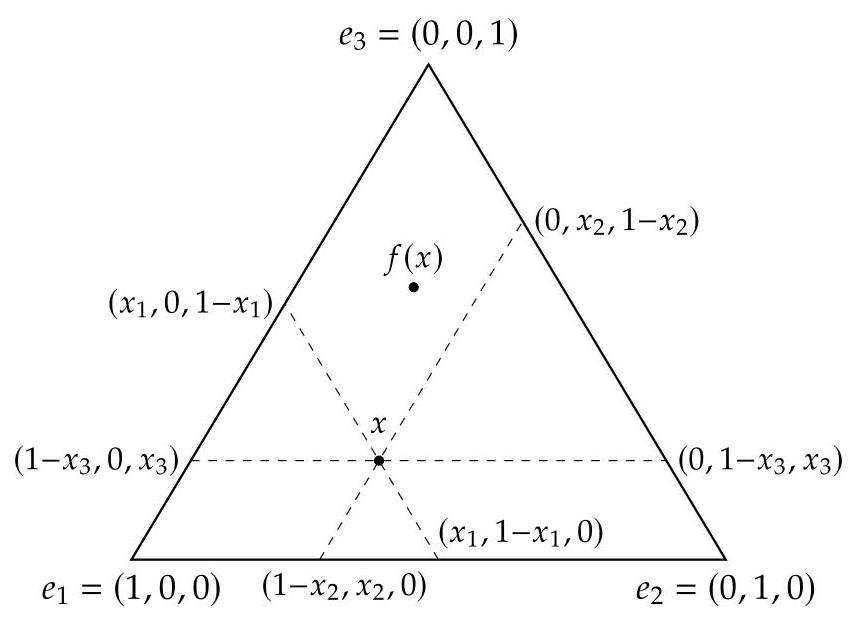
\includegraphics[width=0.6\textwidth]{images/ch07-fig01.jpg}
\caption{对 (\ref{eq:7.2}) 的说明。虚线表示 \(\;\left( {{z}_{1},{z}_{2},{z}_{3}}\right)\) 点，其中 \({z}_{i} = {x}_{i}\) 。这里 \(x\) 有标签 1 和 2，因为 \({x}_{1} \geq {f}_{1}\left( x\right)\) 且 \({x}_{2} \geq {f}_{2}\left( x\right)\) 。}
\label{fig:7.1}
\end{figure}
根据以下规则为每个 \(x \in  \Delta\) 分配

\begin{equation}
x\text{标识 }i \Leftrightarrow  {x}_{i} \geq  {f}_{i}\left( x\right) \;\left( {1 \leq  i \leq  d}\right) \text{ . }\label{eq:7.2}
\end{equation}

\(x = \left( {{x}_{1},\ldots ,{x}_{d}}\right)\) 的任何标签 \(i\) 都标识了 \(x\) 的一个分量 \({x}_{i}\) ，在 \(f\left( x\right)\) 中该分量不会增加(增加意味着向 \(\Delta\) 的顶点 \({e}_{i}\) 移动)；见图\ref{fig:7.1}。

如果 \(x\) 拥有每个标签 \(i \in  \{ 1,\ldots ,d\}\) ，则点 \(x \in  \Delta\) 是完全标记的。这个条件刻画了 \(f\) 的不动点。

\bigskip
\noindent
\begin{lemma}\label{lem:7.1}
设 \(f : \Delta  \rightarrow  \Delta\) 和 \(x \in  \Delta\) 。那么 \(f\left( x\right)  = x\) 当且仅当 \(x\) 是完全标记的。
\end{lemma}

\bigskip
\noindent
\begin{proof}
如果 \(f\left( x\right)  = x\) ，那么对于所有 \(i = 1,\ldots ,d\) 有 \({f}_{i}\left( x\right)  = {x}_{i}\) ，因此 \(x\) 是完全标记的。反之，假设 \(x\) 是完全标记的，对于所有 \(i\) 有 \({x}_{i} \geq  {f}_{i}\left( x\right)\) 。如果对于某个 \(i\) 有 \({x}_{i} > {f}_{i}\left( x\right)\) ，那么 \(\mathop{\sum }\limits_{{k = 1}}^{d}{x}_{k} > \mathop{\sum }\limits_{{k = 1}}^{d}{f}_{k}\left( x\right)  = 1\) ，这与 \(x \in  \Delta\) 矛盾。因此，对于所有 \(i\) 有 \({x}_{i} = {f}_{i}\left( x\right)\) ，即 \(f\left( x\right)  = x\) ，得证。
\end{proof}

我们证明布劳威尔不动点定理的策略如下:

\begin{itemize}
\item 在某种“网格”上用有限个点对 \(\Delta\) 进行离散化。
\end{itemize}

\begin{itemize}
\item 为简单起见，为每个网格点分配一个单一的标签，而不是像 (\ref{eq:7.2}) 中那样分配一组标签，这样在 (\ref{eq:7.2}) 中，“ \(\Leftrightarrow\) ”被替换为“ \(\Rightarrow\) ”。
\end{itemize}

\begin{itemize}
\item 证明存在一组“相邻网格点”，它们共同拥有所有标签，这将定位一个“近似不动点”。
\end{itemize}

\begin{itemize}
\item 通过选择越来越精细的网格，这种近似不动点的合适极限定义了所考虑函数的一个不动点。
\end{itemize}

我们以图6.6中的例子来说明这一策略，其中 \(f\) 定义在 \(\left\lbrack  {0,1}\right\rbrack\) 上。区间 \(\left\lbrack  {0,1}\right\rbrack\) 对应于(\ref{eq:7.1})中 \(d = 2\) 时的 \(\Delta\) ，它是 \({\mathbb{R}}^{2}\) 中连接两点 (1,0) 和 (0,1) 的线段，因为 \(\Delta\) 中的元素 \(\left( {{x}_{1},{x}_{2}}\right)\) 由 \(\left( {1 - {x}_{2},{x}_{2}}\right)\) 唯一给出，其中 \({x}_{2} \in  \left\lbrack  {0,1}\right\rbrack\) 。类似地，我们可以将函数 \(f : \Delta  \rightarrow  \Delta\) 与其第二个分量 \({f}_{2}\left( {{x}_{1},{x}_{2}}\right)\) 等同起来，因为 \({f}_{1}\left( {{x}_{1},{x}_{2}}\right)  = 1 - {f}_{2}\left( {{x}_{1},{x}_{2}}\right)\) 。那么，如果 \({x}_{1} \geq  {f}_{1}\left( {{x}_{1},{x}_{2}}\right)\) 或者等价地 \({x}_{2} \leq  {f}_{2}\left( {1 - {x}_{2},{x}_{2}}\right)\) ，则 \(\left( {{x}_{1},{x}_{2}}\right)\) 的标签为1；如果 \({x}_{2} \geq  {f}_{2}\left( {1 - {x}_{2},{x}_{2}}\right)\) ，则标签为2。此外，我们可以假设

\begin{equation}
\left( {1,0}\right) \text{标记为 }1,\;\left( {0,1}\right) \text{ 标记为 2 . }\label{eq:7.3}
\end{equation}

\begin{figure}[htbp]
\centering
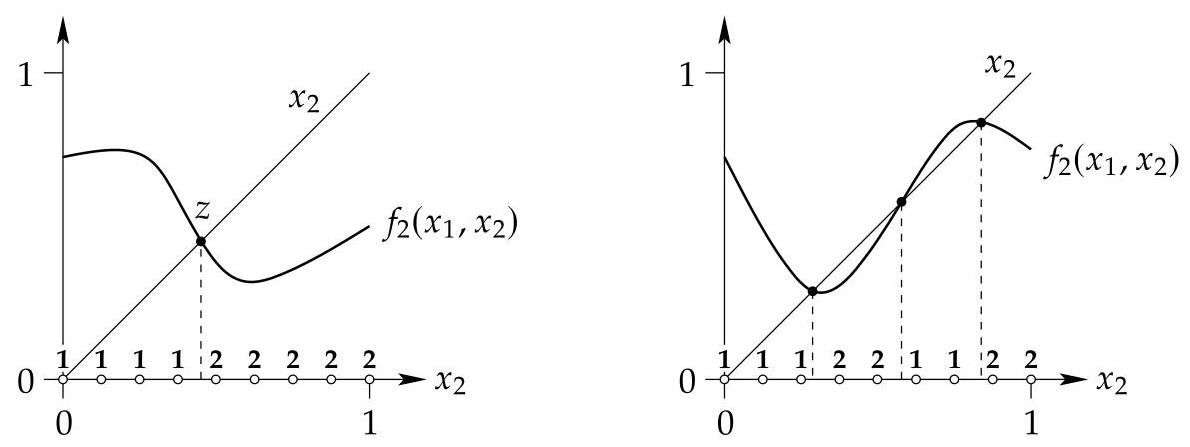
\includegraphics[width=0.9\textwidth]{images/ch07-fig02.jpg}
\caption{\(d = 2\) 时 \(\Delta\) 的标记剖分的两个例子。一个完全标记的子线段包含 \(f\) 的一个不动点。}
\label{fig:7.2}
\end{figure}


图\ref{fig:7.2}的左图展示了图6.6中的例子，线段 \(\Delta\) 表示为包含 \({x}_{2}\) 的区间 \(\left\lbrack  {0,1}\right\rbrack\) 。 \(\Delta\) 中的一些“格点”用白点表示。每个格点根据 \({x}_{2} - {f}_{2}\left( {1 - {x}_{2},{x}_{2}}\right)\) 的符号被赋予一个标签。这些点将 \(\Delta\) 细分为子线段，每个子线段都有一个标记的端点。一个子线段的两个端点分别带有标签1和2，则称其为 {\color{red} 完全被标记} 。这样的子线段包含 \(f\) 的一个不动点 \(z\) ，因为当 \({x}_{2}\) 处于该子区间时， \({x}_{2} - {f}_{2}\left( {1 - {x}_{2},{x}_{2}}\right)\) 的符号会发生变化。在图\ref{fig:7.2}中，条件(\ref{eq:7.3})自动成立，因为 (1,0) 只有标签1，而 (0,1) 只有标签2。一般来说，(\ref{eq:7.3})意味着至少存在一个完全标记的子线段，因为当 \({x}_{2}\) 从0变化到1时，某个格点 \(\left( {1 - {x}_{2},{x}_{2}}\right)\) 的标签会在某一点从1变为2。

在图\ref{fig:7.2}的右图中，函数 \(f\) 有三个不动点，同样由完全标记的子线段确定。在两个图中，使用“更精细”的网格可以更精确地定位不动点。

\section{单纯形与三角剖分}\label{sec-7.3}

在图\ref{fig:7.2}中， \({\mathbb{R}}^{d}\) 中的单位单纯形 \(\Delta\) 是一个线段，它被细分为更小的子线段。对于一般的 \(d\) ，这种情况的推广是将 \(\Delta\) 细分为更小的子单纯形，称为单纯剖分或三角剖分，它将起到所指示的“网格”的作用。

我们需要的几何学基本操作是，在 \({\mathbb{R}}^{d}\) 中过两点 \(x\) 和 \(y\) 画一条直线，如图5.4所示，并重复这个过程(不在该直线上的第三点与直线上的任意一点可确定一个平面，依此类推)。过 \(x\) 和 \(y\) 的直线上的点是形如 \(x\left( {1 - \lambda }\right)  + {y\lambda }\) (其中 \(\lambda  \in  \mathbb{R}\) )的特殊线性组合，称为仿射组合。一般地， \({\mathbb{R}}^{d}\) 中各点 \({v}^{1},\ldots ,{v}^{n}\) 的仿射组合形式为 \(\mathop{\sum }\limits_{{i = 1}}^{n}{v}^{i}{\lambda }_{i}\) ，其中 \({\lambda }_{1},\ldots ,{\lambda }_{n}\) 为实数且满足 \(\mathop{\sum }\limits_{{i = 1}}^{n}{\lambda }_{i} = 1\) 。若对于 \(1 \leq  i \leq  n\) 有 \({\lambda }_{i} \geq  0\) ，则称其为凸组合。如果一个点集在形成凸组合时是封闭的，那么该点集就是凸集。点集 \(V\) 的凸包 \(conv~ V\) 是(关于集合包含关系)包含 \(V\) 的最小凸集 \(C\) ，即 \(V \subseteq  C\) 。

若给定的点集中没有一个点是其他点的仿射组合，则这些点是仿射无关的。这可以通过高一维的线性无关性给出一个简单的等价刻画。

\bigskip
\noindent
\begin{lemma}\label{lem:7.2}
\({\mathbb{R}}^{d}\) 中的向量 \({v}^{1},\ldots ,{v}^{n}\) 仿射无关当且仅当

向量

\begin{equation}
\left( \begin{array}{l} 1 \\  {v}^{1} \end{array}\right) ,\ldots ,\left( \begin{matrix} 1 \\  {v}^{n} \end{matrix}\right)\label{eq:7.4}
\end{equation}

在 \({\mathbb{R}}^{1 + d}\) 中线性无关。
\end{lemma}

\bigskip
\noindent
\begin{proof}
假设 \({\mathbb{R}}^{d}\) 中的 \({v}^{1},\ldots ,{v}^{n}\) 不是仿射无关的。也就是说，某个向量，比如 \({v}^{1}\) ，是其他向量的仿射组合，存在实数 \({\lambda }_{2},\ldots ,{\lambda }_{n}\) 使得

\[
1 = {\lambda }_{2} + \cdots  + {\lambda }_{n}
\]

\[
{v}^{1} = {v}^{2}{\lambda }_{2} + \cdots  + {v}^{n}{\lambda }_{n}.
\]

这等价于

\begin{equation}
\left( \begin{matrix} 1 \\  {v}^{1} \end{matrix}\right) \left( {-1}\right)  + \left( \begin{matrix} 1 \\  {v}^{2} \end{matrix}\right) {\lambda }_{2} + \cdots  + \left( \begin{matrix} 1 \\  {v}^{n} \end{matrix}\right) {\lambda }_{n} = \left( \begin{array}{l} 0 \\  \mathbf{0} \end{array}\right)\label{eq:7.5}
\end{equation}

这表明(\ref{eq:7.4})中的向量不是线性无关的。反之，如果它们不是线性无关的，即

\begin{equation}
\left( \begin{matrix} 1 \\  {v}^{1} \end{matrix}\right) {\lambda }_{1} + \left( \begin{matrix} 1 \\  {v}^{2} \end{matrix}\right) {\lambda }_{2} + \cdots  + \left( \begin{matrix} 1 \\  {v}^{n} \end{matrix}\right) {\lambda }_{n} = \left( \begin{array}{l} 0 \\  \mathbf{0} \end{array}\right)\label{eq:7.6}
\end{equation}

其中 \({\lambda }_{1},\ldots ,{\lambda }_{n}\) 不全为零，不妨设 \({\lambda }_{1} \neq  0\) ，那么用 \(- 1/{\lambda }_{1}\) 乘以(\ref{eq:7.6})式就得到(\ref{eq:7.5})式，从而说明 \({v}^{1},\ldots ,{v}^{n}\) 是仿射相关的。((\ref{eq:7.4})中额外的第一行元素都为1是为了保证线性无关性，例如当某个 \({v}^{i}\) 是零向量时，零向量在仿射组合中没有特殊作用。)
\end{proof}

一个凸集的维度为 \(n\) 当且仅当它有 \(n + 1\) 个但不会更多的仿射无关点。有界多面体是某个欧几里得空间 \({\mathbb{R}}^{d}\) 中有限点集的凸包。如果这些点是仿射无关的，那么这个有界多面体就称为单纯形。

式\eqref{eq:7.1}中的单位单纯形 \(\Delta\) 是 \({\mathbb{R}}^{d}\) 中单位向量 \({e}_{1},\ldots ,{e}_{d}\) 的凸包。它们仿射无关，因此单位单纯形的维度为 \(d - 1\) ，出于这个原因，它有时用 \({\Delta }_{d - 1}\) 表示。例如(见图\ref{fig:7.1})， \({\Delta }_{2}\) 是 \({\mathbb{R}}^{3}\) 中三个单位向量的凸包，是一个三角形，其维度为2(尽管它是 \({\mathbb{R}}^{3}\) 的子集，因为 \({\Delta }_{2}\) 中的所有 \({\left( {x}_{1},{x}_{2},{x}_{3}\right) }^{\top }\) 都满足方程 \(\left. {{x}_{1} + {x}_{2} + {x}_{3} = 1}\right)\) )。

根据维度的定义，空集的维度为 -1。维度为零的集合是任何单元素集。一维单纯形是两个不同点的凸包，因此是一条线段。二维单纯形是一个三角形。三维单纯形是一个四面体。给定维度的每个单纯形(在任何可能维度大得多的欧几里得空间中)都与相同维度的单位单纯形存在仿射(因此是连续的)双射，如下所示。

\bigskip
\noindent
\begin{lemma}\label{lem:7.3}
设 \(S\) 是一个维度为 \(d - 1\) 的单纯形，它是某个 \({\mathbb{R}}^{k}\) 中仿射无关点 \({v}^{1},\ldots ,{v}^{d}\) 的凸包。那么存在一个线性映射 \({\mathbb{R}}^{d} \rightarrow  {\mathbb{R}}^{k}\) ，其在式\eqref{eq:7.1}中 \(\Delta\) 上是一个双射 \(\Delta  \rightarrow  S\) 。其逆 \(J : S \rightarrow  \Delta\) 是一个从\({\mathbb{R}}^{k} \rightarrow  {\mathbb{R}}^{d}\)的仿射映射。
\end{lemma}

\bigskip
\noindent
\begin{proof}
如果 \(x \in  S\) ，那么存在非负实数 \({\lambda }_{1},\ldots ,{\lambda }_{d}\) 使得

\begin{equation}
\left( \begin{array}{l} 1 \\  x \end{array}\right)  = \left( \begin{matrix} 1 \\  {v}^{1} \end{matrix}\right) {\lambda }_{1} + \cdots  + \left( \begin{matrix} 1 \\  {v}^{d} \end{matrix}\right) {\lambda }_{d}\label{eq:7.7}
\end{equation}

由仿射无关性和引理\ref{lem:7.2}可知，式\eqref{eq:7.7}中的系数向量 \(\lambda  = {\left( {\lambda }_{1},\ldots ,{\lambda }_{d}\right) }^{\top }\) 是唯一的，不同的系数向量定义不同的点 \(x \in  S\) 。这些系数向量 \(\lambda\) 属于单位单纯形 \(\Delta\) ，因此通过式\eqref{eq:7.7}中的线性映射 \(\lambda  \mapsto  x\) 与 \(\Delta  \rightarrow  S\) 存在双射。
\end{proof}

可以看出，这个双射的逆是如下仿射映射 \({\mathbb{R}}^{k} \rightarrow  {\mathbb{R}}^{d}\) 。我们首先构造一个线性映射 \({\mathbb{R}}^{1 + k} \rightarrow  {\mathbb{R}}^{d}\) ，它由其在 \({\mathbb{R}}^{1 + k}\) 的一组基上的(任意)像唯一确定。为此，将 \(\left( \begin{matrix} 1 \\  {v}^{1} \end{matrix}\right) ,\ldots ,\left( \begin{matrix} 1 \\  {v}^{d} \end{matrix}\right)\) 扩充为这样一组基，对于 \(1 \leq  i \leq  d\) ，将 \(\left( \begin{matrix} 1 \\  {v}^{i} \end{matrix}\right)\) 映射到 \({\mathbb{R}}^{d}\) 中的单位向量 \({e}_{i}\) ，并将其余每个基向量映射到 0。因为这是一个线性映射，所以对于某个 \(d \times  \left( {1 + k}\right)\) 矩阵 \(A\) ，它可以写成 \(\left( \begin{array}{l} \alpha \\  x \end{array}\right)  \mapsto  \lambda  = A\left( \begin{array}{l} \alpha \\  x \end{array}\right)\) (其中 \(\alpha  \in  \mathbb{R}\) 且 \(x \in  {\mathbb{R}}^{k}\) )。根据 (\ref{eq:7.7})，若 \(\alpha  = 1\) 且 \(x \in  S\) ，则 \(\lambda  \in  \Delta\) 。对于 \(\alpha  = 1\) ，我们得到一个仿射映射 \({\mathbb{R}}^{k} \rightarrow  {\mathbb{R}}^{d}\) ，即 \(x \mapsto  \lambda  = A\left( \begin{array}{l} 1 \\  x \end{array}\right)\) 。这个映射限制在 \(S\) 上就是所需的仿射双射 \(J : S \rightarrow  \Delta\) 。(若 \(x \notin  S\) ，则 \(A\left( \begin{array}{l} 1 \\  x \end{array}\right)\) 依赖于额外基向量的选取，所以 \(A\) 本身不是唯一的，但这在这里无关紧要；限制映射 \(J : S \rightarrow  \Delta\) 是唯一的。)

在 (\ref{eq:7.7}) 中，唯一的系数 \({\lambda }_{1},\ldots ,{\lambda }_{d}\) 被称为 \(x\) 在 \(S\) 中的重心坐标(它依赖于定义单纯形 \(S\) 的点 \({v}^{1},\ldots ,{v}^{d}\) 的选取顺序)。“重心”这个名称的由来是，对于 \(1 \leq  i \leq  d\) ， \(x\) 是放置在点 \({v}^{i}\) 处权重为 \({\lambda }_{i}\) 的加权重心。

考虑一个维度为 \(d - 1\) 的单纯形 \(S\) ，它是 \(d\) 个仿射无关点 \({v}^{1},\ldots ,{v}^{d}\) 的凸包。那么这些点的任何子集(包括空集)也是仿射无关的，并且其凸包也是一个单纯形。每个这样的单纯形都称为 \(S\) 的一个面。任何单元素面 \(\left\{  {v}^{i}\right\}\) 或 \({v}^{i}\) 本身都称为 \(S\) 的一个顶点。维度为 1 的面称为一条边。 \(S\) 中维度为 \(d - 2\) 的面称为 \(S\) 的一个极面。一般有界多面体 \(P\) 的一个顶点 \(v\) 是 \(P\) 的一个极点，即 \(v \in  P\) 且 \(v\) 不是 \(P\) 中其他点的凸组合。练习~\ref{exer:7.2} 表明，单纯形的每个顶点确实是这样一个极点。

\bigskip
\noindent
\begin{definition}\label{def:7.4}
设 \(P\) 为一个有界多面体。 \(P\) 的一个三角剖分或单纯剖分是一个由子单纯形 \({S}_{i}\) 组成的有限集合 \(\sum  = \left\{  {{S}_{1},\ldots ,{S}_{N}}\right\}\) ，其中 \(i = 1,\ldots ,N\) 满足:(a) \(P = \mathop{\bigcup }\limits_{{i = 1}}^{N}{S}_{i}\) ；(b) 没有一个子单纯形是另一个子单纯形的子集；(c) 任意两个子单纯形的交集是这两个子单纯形的一个面。 \(\sum\) 中的一个顶点是 \(\sum\) 中任意一个子单纯形的任意一个顶点。 \(\sum\) 中的一个子极面(sub - facet)是 \(\sum\) 中任意一个子单纯形的任意一个极面。
\end{definition}

\begin{figure}[htbp]
\centering
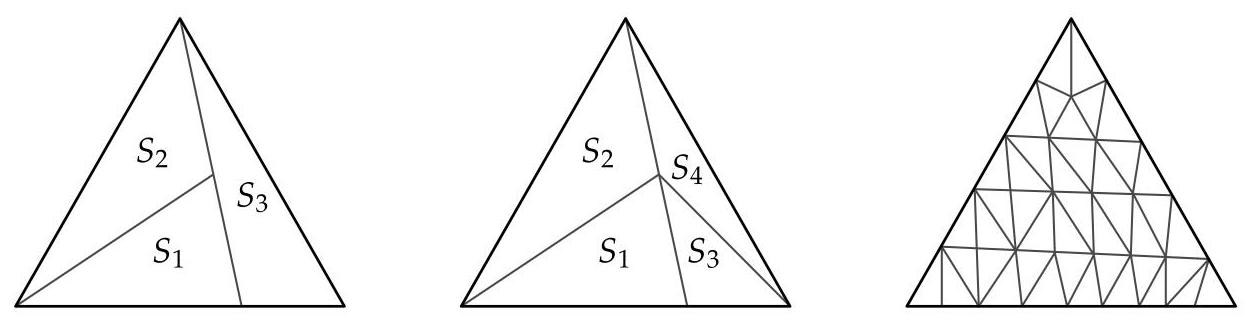
\includegraphics[width=0.9\textwidth]{images/ch07-fig03.jpg}
\caption{左图: \(\left\{ {{S}_{1},{S}_{2},{S}_{3}}\right\}\) 不是该三角形的一个三角剖分，因为 \({S}_{1} \cap {S}_{3}\) 不是 \({S}_{3}\) 的一个面。中图和右图:该三角形的三角剖分。}
\label{fig:7.3}
\end{figure}


在定义\ref{def:7.4}(c)中，两个子单纯形的交集可能是空集，空集是任意有界多面体的一个面。图\ref{fig:7.3}展示了三角形的单纯剖分的概念。左图满足定义\ref{def:7.4}的条件(a)和(b)，但不满足条件(c)，而中图满足条件(c)。右图表明，三角剖分中的子单纯形的形状和大小可以不同。

以下引理陈述了三角剖分的一些相当直观的性质。

\bigskip
\noindent
\begin{lemma}\label{lem:7.5}
设 \(S\) 是一个顶点为 \({v}^{1},\ldots ,{v}^{d}\) 的单纯形， \(\sum\) 是 \(S\) 的一个三角剖分。那么 \(\sum\) 中的所有子单纯形 \({S}_{i}\) 与 \(S\) 具有相同的维度\(d - 1\) 。
\end{lemma}

\bigskip
\noindent
\begin{proof}
任意子单纯形的顶点都属于 \(S\) ， \(S\) 的维度为 \(d - 1\) ，所以没有子单纯形的维度可以更高。假设一个子单纯形，称它为 \({S}_{1}\) ，维度更低，其顶点为 \({w}^{1},\ldots ,{w}^{k}\) 和 \(k < d\) 。设 \(x = \mathop{\sum }\limits_{{i = 1}}^{k}{w}^{i}\frac{1}{k}\) 是 \({S}_{1}\) 的重心。 \(S\) 中至少有一个顶点 \({v}^{i}\) 不是 \({w}^{1},\ldots ,{w}^{k}\) 的仿射组合。对于 \(\varepsilon  \in  \mathbb{R}\) ，设

\begin{equation}
z\left( \varepsilon \right)  = x\left( {1 - \varepsilon }\right)  + {v}^{i}\varepsilon .\label{eq:7.8}
\end{equation}

从几何角度看，点 \(z\left( \varepsilon \right)\) 位于过 \(x\) 和 \({v}^{i}\) 的直线上，见图\ref{fig:7.4}。

\begin{figure}[htbp]
\centering
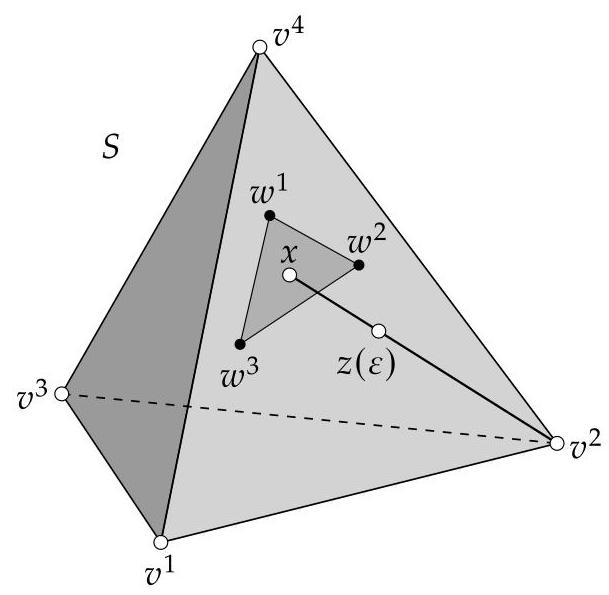
\includegraphics[width=0.4\textwidth]{images/ch07-fig04.jpg}
\caption{展示了(\ref{eq:7.8})式对于 \(d = 4,k = 3\) 以及(\ref{eq:7.9})式中 \(i = 2\) 的情况。}
\label{fig:7.4}
\end{figure}

那么对于 \(\varepsilon  \neq  0\) ，我们有 \({v}^{i} = z\left( \varepsilon \right) \frac{1}{\varepsilon } + x\left( {1 - \frac{1}{\varepsilon }}\right)\) ，这表明 \(z\left( \varepsilon \right)\) 不是 \({w}^{1},\ldots ,{w}^{k}\) 的仿射组合，因为否则 \({v}^{i}\) 也会是。也就是说，

\begin{equation}
z\left( \varepsilon \right)  \notin  {S}_{1}\;\left( {\varepsilon  \neq  0}\right) .\label{eq:7.9}
\end{equation}

考虑在 \((0,1\rbrack\) 中的一个递减序列 \({\varepsilon }_{1},{\varepsilon }_{2},\ldots\) ，它趋于 0，例如 \({\varepsilon }_{n} = \frac{1}{n}\) ，根据 (\ref{eq:7.8}) 式，因为 \(S\) 是凸集，所以 \(z\left( {\varepsilon }_{n}\right)  \in  S\) 。由于 \(S\) 是 \(\sum\) 中子单纯形的并集，对于每个 \(n\) ，存在某个子单纯形包含 \(z\left( {\varepsilon }_{n}\right)\) 。因为 \(\sum\) 是有限的，所以有一个子单纯形，记为 \({S}_{2}\) ，包含序列中无限多个点 \(z\left( {\varepsilon }_{n}\right)\) (实际上，该序列中介于这些点之间的所有点也在其中，因为它们在一条线段上，且 \({S}_{2}\) 是凸集)。由于当 \(n \rightarrow  \infty\) 时 \({\varepsilon }_{n} \rightarrow  0\) ，点 \(z\left( {\varepsilon }_{n}\right)\) 收敛于 \(x\) ，这意味着 \(x \in  {S}_{2}\) ，因为 \({S}_{2}\) 是闭集。因此， \(x \in  {S}_{1} \cap  {S}_{2}\) 。根据定义\ref{def:7.4} 中的条件 (c)，交集 \({S}_{1} \cap  {S}_{2}\) 是 \({S}_{1}\) 和 \({S}_{2}\) 的一个面，它包含 \({S}_{1}\) 的所有顶点\({w}^{1},\ldots ,{w}^{k}\) ，因为在表示式 \(x = \mathop{\sum }\limits_{{i = 1}}^{k}{w}^{i}\frac{1}{k}\) 中它们的权重 \(\frac{1}{k}\) 为正。因此， \({S}_{1} = {S}_{1} \cap  {S}_{2}\) ，即 \({S}_{1} \subseteq  {S}_{2}\) 。此外，对于某个 \(\varepsilon  > 0\) 有 \(z\left( \varepsilon \right)  \in  {S}_{2} - {S}_{1}\) ，这意味着 \({S}_{1} \neq  {S}_{2}\) 。这与定义\ref{def:7.4}(b) 矛盾。因此，如前所述，所有子单纯形的维度 \(d - 1\) 都与 \(S\) 相同。
\end{proof}


\bigskip
\noindent
\begin{lemma}\label{lem:7.6}
设 \(S\) 为一个单纯形， \(\sum\) 为 \(S\) 的一个三角剖分， \(F\) 为 \(\sum\) 中的一个子极面。则以下两种情况恰好发生其一:

(a) \(F\) 是 \(S\) 的一个极面(facet)的子集，且 \(F\) 是 \(\sum\) 中恰好一个子单纯形的极面。

(b) \(F\) 不是 \(S\) 的一个极面的子集，且 \(F\) 是 \(\sum\) 中恰好两个子单纯形的极面。
\end{lemma}

\bigskip
\noindent
\begin{proof}
设 \(S\) 的维度为 \(d - 1\) ，顶点为 \({v}^{1},\ldots ,{v}^{d}\) 。根据引理\ref{lem:7.5}，每个子单纯形的维度也为 \(d - 1\) 。设 \(F\) 是 \(\sum\) 中某个子单纯形 \(T\) 的一个极面， \({w}^{1},\ldots ,{w}^{d - 1}\) 是 \(F\) 的顶点。设 \(x = \mathop{\sum }\limits_{{i = 1}}^{{d - 1}}{w}^{i}\frac{1}{d - 1}\) 是 \(F\) 的重心， \({w}^{d}\) 是 \(T\) 剩下的那个顶点。考虑过 \(x\) 和 \({w}^{d}\) 的直线，该直线上的点为

\[
y\left( \varepsilon \right)  = x\left( {1 - \varepsilon }\right)  + {w}^{d}\varepsilon
\]

对于 \(\varepsilon  \in  \mathbb{R}\) ，其中对于 \(\varepsilon  \in  \left\lbrack  {0,1}\right\rbrack\) 属于 \(T\) 。假设 \(F\) 是另一个子单纯形 \({T}^{\prime }\) 的极面，该子单纯形有另一个第 \(d\) 个顶点 \({w}_{0}\) ，不同于 \({w}_{d}\) 。 \({T}^{\prime }\) 的 \(d\) 个顶点 \({w}^{0},{w}^{1},\ldots ,{w}^{d - 1}\) 仿射无关。因此，存在唯一的 \({\lambda }_{0},{\lambda }_{1},\ldots ,{\lambda }_{d - 1}\) 满足 \({w}^{d} = \mathop{\sum }\limits_{{i = 0}}^{{d - 1}}{w}^{i}{\lambda }_{i}\) ，其中 \({\lambda }_{0} \neq  0\) 是因为 \({w}^{d} \notin  F\) 。我们断言 \({\lambda }_{0} < 0\) ，即 \({w}_{0}\) 和 \({w}_{d}\) 在极面 \(F\) 的两侧。即

\[
y\left( \varepsilon \right)  = x\left( {1 - \varepsilon }\right)  + \mathop{\sum }\limits_{{i = 0}}^{{d - 1}}{w}^{i}{\lambda }_{i}\varepsilon
\]

\[
= {w}^{0}{\lambda }_{0}\varepsilon  + \mathop{\sum }\limits_{{i = 1}}^{{d - 1}}{w}^{i}\left( {\frac{1}{d - 1}\left( {1 - \varepsilon }\right)  + {\lambda }_{i}\varepsilon }\right)
\]

\begin{equation}
= {w}^{0}{\lambda }_{0}\varepsilon  + \mathop{\sum }\limits_{{i = 1}}^{{d - 1}}{w}^{i}\left( {\frac{1}{d - 1} + \left( {{\lambda }_{i} - \frac{1}{d - 1}}\right) \varepsilon }\right) .\label{eq:7.10}
\end{equation}

如果 \({\lambda }_{0} > 0\) ，对于足够小的正 \(\varepsilon\) ，这将意味着 \(y\left( \varepsilon \right)  \in  \left( {T \cap  {T}^{\prime }}\right)  - F\) ，但这是不可能的，因为 \(T\) 和 \({T}^{\prime }\) 在一个公共极面相交，而这个公共极面只能是 \(F\) 。因此，如所断言的 \({\lambda }_{0} < 0\) 。

以下展示了情况 (a) 和 (b)。如果 \(F\) 是 \(S\) 的一个极面的子集，那么对于所有 \(\varepsilon  < 0\) 有 \(y\left( \varepsilon \right)  \notin  S\) :否则，对于 \(\varepsilon  < 0\) 使得 \(y\left( \varepsilon \right)\) 和 \(y\left( {-\varepsilon }\right)\) 在 \(S\) 中，我们有 \(x = y\left( \varepsilon \right) \frac{1}{2} + y\left( {-\varepsilon }\right) \frac{1}{2} = \mathop{\sum }\limits_{{i = 1}}{v}^{i}{\mu }_{i}\) ，其中对于所有 \(i = 1,\ldots ,d\) 有 \({\mu }_{i} > 0\) ，即 \(x\) 在 \(S\) 的内部而不是在 \(S\) 的一个极面上。这意味着不存在如上述所考虑的以 \(F\) 为极面的第二个子单纯形 \({T}^{\prime }\) ，因为 \({T}^{\prime }\) (进而 \(S\) )会包含这样的 \(y\left( \varepsilon \right)\) ，其中有 \(\varepsilon  < 0\) 和 \({\lambda }_{0} < 0\) (根据 (\ref{eq:7.10}))。所以如 (a) 中所述，子单纯形 \(T\) 是唯一的。

另一方面，如果 \(F\) 不是 \(S\) 的一个极面的子集，那么 \(x\) 在 \(S\) 的内部，并且对于 \(\varepsilon  < 0\) 存在 \(y\left( \varepsilon \right)\) 在 \(S\) 中，因此存在以 \(F\) 为极面的第二个子单纯形 \({T}^{\prime }\) 。通过对 \(T\) 应用的相同推理，不存在其他子单纯形，其顶点与 \({T}^{\prime }\) 的顶点 \({w}^{0}\) 在 \(F\) 的同一侧。这展示了情况 (b)，并且显然情况 (a) 或 (b) 中恰好有一种情况成立。
\end{proof}

以下引理将用于下一节的归纳证明。

\bigskip
\noindent
\begin{lemma}\label{lem:7.7}
设 \(n \geq  2\) ，设 \(S\) 为一个顶点为 \({v}^{1},\ldots ,{v}^{n}\) 的单纯形，设 \(F\) 为 \(S\) 中顶点为 \({v}^{1},\ldots ,{v}^{n - 1}\) 的极面，设 \(\sum\) 为 \(S\) 的一个三角剖分，设 \({\sum }^{\prime }\) 为 \(\sum\) 中作为 \(F\) 子集的子极面的集合。那么 \({\sum }^{\prime }\) 是 \(F\) 的一个三角剖分。
\end{lemma}

\bigskip
\noindent
\begin{proof}
设 \({\sum }_{1} = \{ T \cap  F \mid  T \in  \sum \}.\) 那么 \(F = \mathop{\bigcup }\limits_{{{T}^{\prime } \in  {\sum }_{1}}}{T}^{\prime }\) ，因为 \(F\) 中的每个 \(x\) (作为 \(S\) 的一个元素)都属于 \(\sum\) 中的某个子单纯形 \(T\) 。对于每个 \(T \in  \sum\) ，我们断言 \(T \cap  F\) 是 \(T\) 的一个面。即， \(T\) 的每个顶点 \(v\) 都是 \(S\) 的顶点 \({v}^{i}\) 的唯一凸组合 \(v = \mathop{\sum }\limits_{{i = 1}}^{n}{v}^{i}{\lambda }_{i}\) ，其中当且仅当 \({\lambda }_{n} = 0\) 时 \(v \in  F\) 。那么 \(T \cap  F\) 是这些属于 \(F\) 的顶点 \(v\) 的凸包。因此，如所断言， \(T \cap  F\) 是 \(T\) 的一个面，并且是一个维度至多为 \(n - 2\) 的单纯形。

设 \({\sum }_{2}\) 为 \({\sum }_{1}\) 中维度为 \(n - 2\) 的那些单纯形的集合。根据引理\ref{lem:7.5}，由于 \(\sum\) 中的所有单纯形的维度都是 \(n - 1\) ，所以 \({\sum }_{2} = {\sum }^{\prime }\) 。

我们证明每个 \(x \in  F\) 都属于 \({\sum }^{\prime }\) 中的某个单纯形 \({T}^{\prime }\) ，即属于 \({\sum }_{2}\) 。假设存在某个 \(x \in  F\) 不满足该情况。那么对于某个单纯形 \({S}_{1} \in  {\sum }_{1}\) 有 \(x \in  {S}_{1}\) ，其中 \({S}_{1}\) 的维度小于 \(n - 2\) 。设 \({S}_{1}\) 为 \({\sum }_{1}\) 中包含 \(x\) 的最大维度(根据假设至多为 \(n - 3\) )的单纯形。通过与引理\ref{lem:7.5}证明中使用 \(d = n - 1\) 时相同的论证，存在某个 \({S}_{2} \in  {\sum }_{1}\) 是 \({S}_{1}\) 的超集，且比 \({S}_{1}\) 至少多一个顶点且维度更高，这产生矛盾。这表明如所断言 \(F = \mathop{\bigcup }\limits_{{{T}^{\prime } \in  {\sum }^{\prime }}}{T}^{\prime }\) 。

在 \({\sum }^{\prime }\) 中没有两个子极面使得一个是另一个的子集，因为它们具有相同的维度但顶点集不同。此外，两个这样的子极面的交集由它们顶点的交集确定，因此是这两个子极面的一个面。这表明 \({\sum }^{\prime }\) 是 \(F\) 的一个三角剖分。
\end{proof}

\begin{figure}[htbp]
\centering
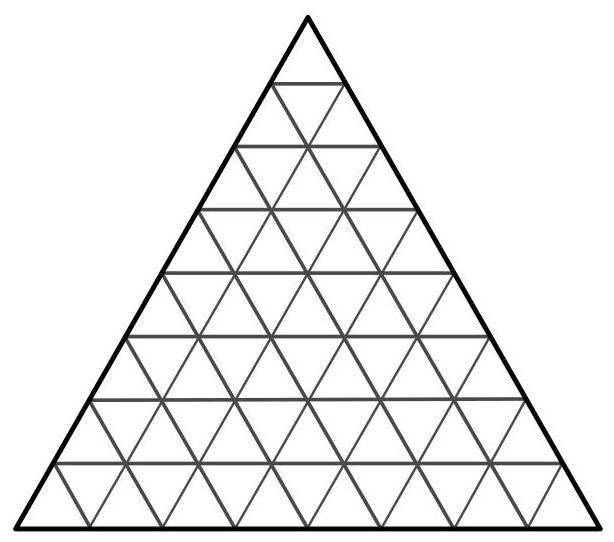
\includegraphics[width=0.4\textwidth]{images/ch07-fig05.jpg}
\caption{正三角形划分为小的相似三角形的三角剖分。}
\label{fig:7.5}
\end{figure}


单纯形 \(S\) 的三角剖分起到了前面提到的“网格”的作用，其顶点即为网格点。目标是能够为任意 \(\varepsilon  > 0\) 创建一个“ \(\varepsilon\) -精细网格”，使得每个子单纯形中的顶点之间的距离不超过 \(\varepsilon\) 。图\ref{fig:7.5}展示了当 \(S\) 为三角形时实现这一目标的一种好方法。然而，对高维单纯形进行三角剖分以达到这一要求并非易事。例如，考虑一个正四面体，它的每个极面(即三角形)被细分为四个正三角形，这些正三角形是通过连接四面体每条边的中点得到的。然后，“切掉”每个角上的小四面体后，会留下一个中心有界多面体，它不是四面体，而是八面体。这个八面体必须以某种新的方式进一步细分为四面体。此外，目前尚不清楚这种构造如何扩展到更高维度。目前，我们假设在任何维度下，我们都能找到单纯形的足够“精细”的三角剖分。实现这一目标的具体构造方法将在第\ref{sec-7.7}节中介绍。

\section{斯佩纳引理}\label{sec-7.4}

在本节中，我们将证明斯佩纳引理，它常被称为布劳威尔不动点定理的组合版本，并且是证明该定理的关键一步。斯佩纳引理适用于具有 \(d\) 个顶点的单纯形 \(S\) 以及 \(S\) 的三角剖分 \(\sum\) ，其中 \(\sum\) 中的每个顶点都被赋予了 \(\{ 1,\ldots ,d\}\) 中的一个标签，且满足以下条件。

\bigskip
\noindent
\begin{definition}[斯佩纳标号]\label{def:7.8}
设 \(S\) 是一个顶点为 \({v}^{1},\ldots ,{v}^{d}\) 的单纯形， \(\sum\) 是 \(S\) 的三角剖分， \(V\) 是 \(\sum\) 中的顶点集。那么，一个为 \(V\) 中的每个 \(x\) 分配标签的函数 \(V \rightarrow  \{ 1,\ldots ,d\}\) ，若满足每当 \(x = \mathop{\sum }\limits_{{k = 1}}^{d}{v}^{k}{\lambda }_{k}\) 且 \(x\) 的标签为 \(i\) 时，有 \({\lambda }_{i} > 0\) ，则称该函数满足斯佩纳条件，并称其为斯佩纳标号。
\end{definition}

\begin{figure}[htbp]
\centering
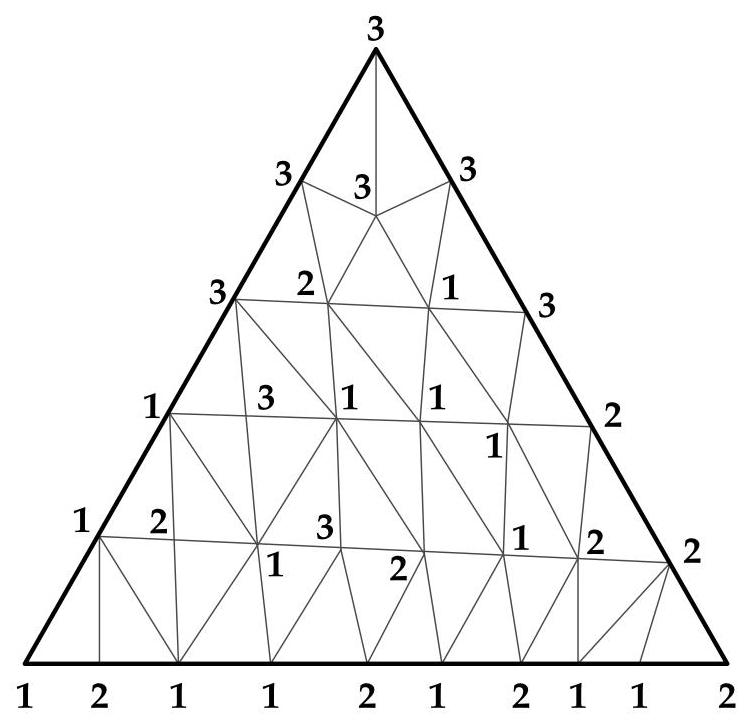
\includegraphics[width=0.5\textwidth]{images/ch07-fig06.jpg}
\caption{带有斯佩纳标号的三角形 \(S\) 的三角剖分。 \(S\) 的顶点 \({v}^{1},{v}^{2},{v}^{3}\) 通过它们各自的标签1、2、3唯一标识。}
\label{fig:7.6}
\end{figure}

请注意，在定义\ref{def:7.8}中，单纯形 \(S\) 中的每个点 \(x\) 都具有如(\ref{eq:7.7})所示的唯一重心坐标 \({\lambda }_{1},\ldots ,{\lambda }_{d}\) 。斯佩纳条件意味着 \(S\) 的每个顶点 \({v}^{i}\) 都有标签 \(i\) (因此每个顶点都有不同的标签)。一般来说，斯佩纳条件规定，如果 \(x\) 位于 \(S\) 的一个面 \(F\) 上(而不是更小的面上)，那么 \(x\) 只能具有 \(F\) 的顶点的标签之一。例如，如果 \(x\) 位于连接 \({v}^{1}\) 和 \({v}^{2}\) 的边上，那么 \(x\) 只能有标签1或2。对于 \(d = 2\) ，斯佩纳条件在(\ref{eq:7.3})中给出。对于 \(d = 3\) ，单纯形 \(S\) 是一个三角形，图\ref{fig:7.6}展示了一个带有斯佩纳标号的三角剖分示例。

对于 (\ref{eq:7.1}) 中单位单纯形 \(f : \Delta  \rightarrow  \Delta\) 上的函数 \(\Delta\) 以及 \(x \in  \Delta\) ，(\ref{eq:7.2}) 中定义的 \(x\) 的标签之一总能被选来满足斯佩纳条件。

\bigskip
\noindent
\begin{lemma}\label{lem:7.9}
考虑 (\ref{eq:7.1}) 中 $(d - 1)$ 维单位单纯形 \(\Delta\) 以及函数 \(f : \Delta  \rightarrow  \Delta\) 。那么每个点 \(x \in  \Delta\) 都可以被赋予一个标签 \(i\) ，使得 \({x}_{i} \geq  {f}_{i}\left( x\right)\) 且斯佩纳条件成立。
\end{lemma}

\bigskip
\noindent
\begin{proof}
因为 \(\Delta\) 是单位向量 \({e}_{1},\ldots ,{e}_{d}\) 的凸包， \(x \in  \Delta\) 的重心坐标就是 \({x}_{1},\ldots ,{x}_{d}\) 。设 \(I = \left\{  {i \mid  {x}_{i} > 0}\right\}\) 。如果对于所有 \(i \in  I\) 都有 \({f}_{i}\left( x\right)  > {x}_{i}\) ，那么

\[
\mathop{\sum }\limits_{{i = 1}}^{d}{f}_{i}\left( x\right)  \geq  \mathop{\sum }\limits_{{i \in  I}}{f}_{i}\left( x\right)  > \mathop{\sum }\limits_{{i \in  I}}{x}_{i} = \mathop{\sum }\limits_{{i = 1}}^{d}{x}_{i} = 1,
\]

这与 \(f\left( x\right)  \in  \Delta\) 矛盾。所以至少存在一个 \(i \in  I\) 使得 \({x}_{i} \geq  {f}_{i}\left( x\right)\) ，即 \({x}_{i} > 0\) 且 \(x\) 具有标签 \(i\) ，符合要求。
\end{proof}

斯佩纳引理断言，带有斯佩纳标号的单纯形的三角剖分至少有一个完全标记的子单纯形。一个合适的归纳证明可以得出更强的结论，即完全标记的子单纯形的数量是奇数。图\ref{fig:7.7} 展示了前面所考虑的细分三角形的这种情况。

\bigskip
\noindent
\begin{theorem}[斯佩纳引理]\label{theo:7.10}
设 \(S\) 是一个顶点为 \({v}^{1},\ldots ,{v}^{d}\) 的单纯形，设 \(\sum\) 是 \(S\) 的一个三角剖分，并考虑 \(V\) 中顶点的斯佩纳标号。那么 \(\sum\) 有奇数个完全标记的子单纯形 \(T\) (即， \(\{ 1,\ldots ,d\}\) 中的每个标签都是 \(T\) 的某个顶点的标签)。
\end{theorem}

\bigskip
\noindent
\begin{proof}
在定理的陈述中， \(S\) 的顶点 \({v}^{1},\ldots ,{v}^{d}\) 可以是任意 \(k \geq  d - 1\) 下某个空间 \({\mathbb{R}}^{k}\) 中的元素。考虑以下陈述:

\bigskip
\noindent
(i) 设 \(1 \leq  n \leq  d\) ，设 \({F}_{n}\) 是顶点为 \({v}^{1},\ldots ,{v}^{n}\) 的单纯形，且设 \({\sum }_{n} = \{ F \mid  F\) 是某个 \(\left. {T \in  \sum \text{的} n - 1 \text{维面} \text{且 }F \subseteq  {F}_{n}}\right \}\)。那么 \({\sum }_{n}\) 是 \({F}_{n}\) 的一个三角剖分。

{\color{red}根据定理\ref{theo:7.10}的叙述}，陈述(i) 对于 \(n = d\) 是成立的。如果 陈述(i) 对于某个 \(n > 1\) 成立，那么引理\ref{lem:7.7}(对应 \(d = n\)情形 )意味着 \({\sum }_{n - 1}\) 是 \({F}_{n - 1}\) 的一个三角剖分。因此，通过归纳法，陈述(i) 对于 \(n = d,d - 1,\ldots ,1\) 均成立。我们现在通过归纳法证明:

\begin{figure}[htbp]
\centering
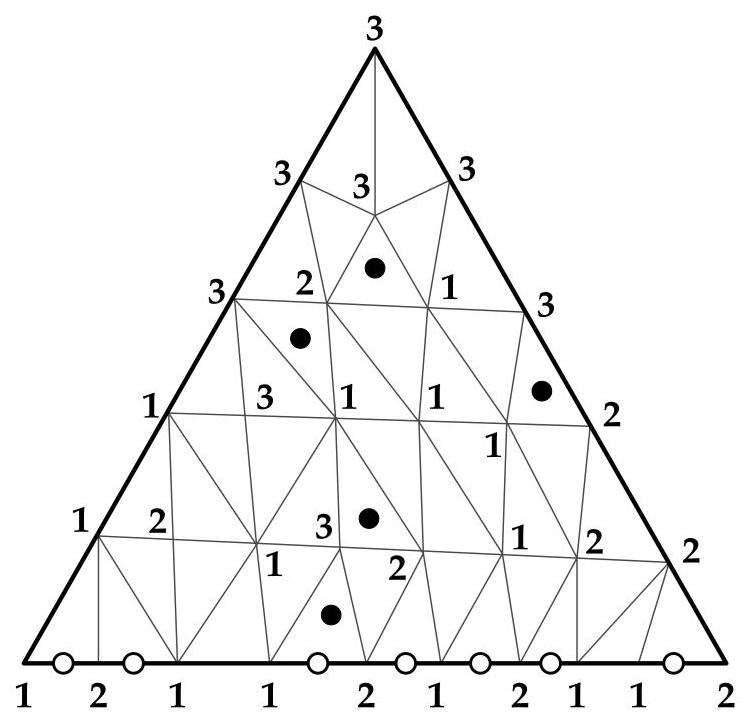
\includegraphics[width=0.5\textwidth]{images/ch07-fig07.jpg}
\caption{斯佩纳引理(定理\ref{theo:7.10})的图示. 黑色(实心)点标记完全标记的子单纯形，白色(空心)点标记完全标记的子极面，如定理\ref{theo:7.10} 的归纳证明中所使用的。白色和黑色点的数量都是奇数。}
\label{fig:7.7}
\end{figure}

\bigskip
\noindent
(ii) 对于 \(n = 1,2,\ldots ,d\) ，设 \({\sum }_{n}\) 为 (i) 中所定义的 \({F}_{n}\) 的三角剖分。若 \(T\) 的顶点具有所有标签 \(1,\ldots ,n\) ，则称 \(T \in  {\sum }_{n}\) 为完全标记的。那么 \({\sum }_{n}\) 有奇数个完全标记的单纯形 \(T\) 。

对于 \(n = 1\) (其中 \({F}_{1} = \left\{  {v}_{1}\right\}\) )，命题 (ii) 是显然的。为了证明归纳步骤，假设 (ii) 对于某个 \(n \geq  1\) (其中 \(n < d\) )成立，我们要证明 (ii) 对于 \(n + 1\) 也成立。对于 \(\sum\) 中单纯形 \(T\) 的任意面 \(F\) ，设

\[
L\left( F\right)  = \{ i \mid  i\text{ 是}F \text{中一些顶点的标签}\} .
\]

考虑以下集合:

\[
C = \left\{  {F \in  {\sum }_{n} \mid  L\left( F\right)  = \{ 1,\ldots ,n\} }\right\}  ,
\]

\begin{equation}
{C}^{\prime } = \left\{  {F \mid  F\text{是一些}T \in  {\sum }_{n + 1}\text{的极面},L\left( F\right)  = \{ 1,\ldots ,n\} ,F \notin  {\sum }_{n}}\right\}  ,\label{eq:7.11}
\end{equation}

\[
D = \left\{  {T \in  {\sum }_{n + 1} \mid  L\left( T\right)  = \{ 1,\ldots ,n + 1\} }\right\}  ,
\]

\[
A = \left\{  {T \in  {\sum }_{n + 1} \mid  L\left( T\right)  = \{ 1,\ldots ,n\} }\right\}  .
\]

情况 \(n = 2\) 如图\ref{fig:7.7} 和 7.8 所示。集合 \({F}_{3} = {F}_{n + 1}\) 是前面考虑的三角形，它有一个将 \({F}_{3}\) 三角剖分成三角形的三角剖分 \({\sum }_{3}\) ； \({\sum }_{3}\) 中的顶点可能具有标签 1、2 和 3。 \({\sum }_{3}\) 中完全标记的元素定义了集合 \(D\) ，并用黑点标记。集合 \({F}_{2} = {F}_{n}\) 是三角形 \({F}_{3}\) 的底部极面，它有一个将 \({F}_{2}\) 三角剖分成线段的三角剖分 \({\sum }_{2}\) ； \({\sum }_{2}\) 中的顶点可能具有标签 1 和 2。 \({\sum }_{2}\) 中完全标记的元素定义了集合 \(C\) ，并用白点标记。根据归纳假设， \(\left| C\right|\) 是奇数。

集合 \({C}^{\prime }\) 是子极面 \(F\) 的集合，其 \(n\) 个顶点具有所有标签 \(1,\ldots ,n\) 且不在 \({\sum }_{n}\) 中；在图\ref{fig:7.8} 中，它们也用白点标记。(当 \(n + 1 = d\) 时，我们使用这样的术语，称 \({\sum }_{n + 1}\) 的元素为“子单纯形”，子单纯形的任何极面为“子极面”，这包括 \({\sum }_{n}\) 的元素。)集合 \(A\) 是几乎完全标记的子单纯形的集合，对于任意 \(T \in  A\) ， \(T\) 的 \(n + 1\) 个顶点具有所有标签 \(1,\ldots ,n\) 但不具有标签 \(n + 1\) 。

\begin{figure}[htbp]
\centering
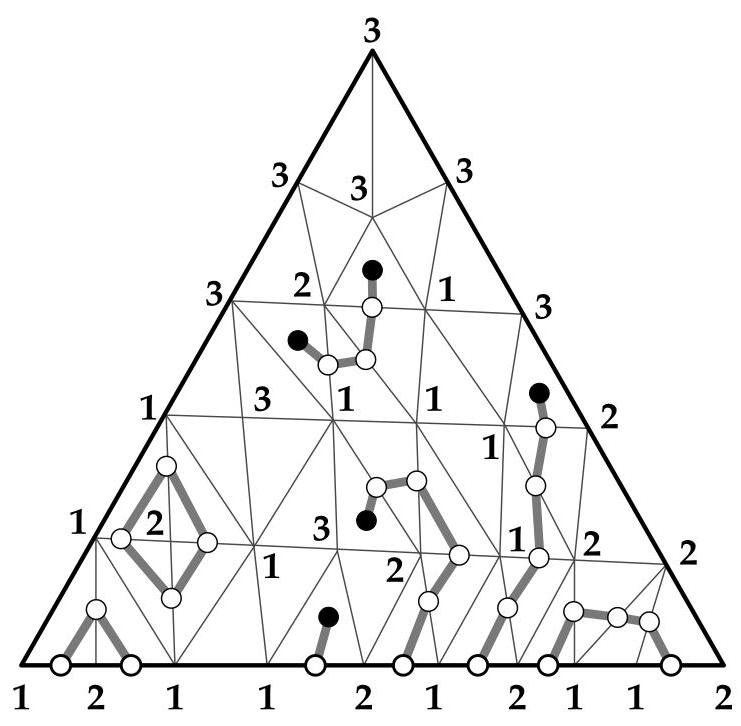
\includegraphics[width=0.5\textwidth]{images/ch07-fig08.jpg}
\caption{为 \(n = 2\) 定义的集合 (\ref{eq:7.11})。 \(C\) 的元素(白点)在 \({\sum }_{2}\) 中，标签为 1、2， \(D\) 的元素(黑点)是 \({\sum }_{3}\) 中的子单纯形，标签为 1、2、3。它们通过路径相连，路径上还有 \({C}^{\prime }\) 中的其他节点(白点，三角形内标签为 1、2 的子极面)，这些定义了图 \({G}_{3}\) 。因此， \(\left| {C \cup D}\right|\) 是偶数，由于 \(\left| C\right|\) 是奇数，所以 \(\left| D\right|\) 是奇数。}
\label{fig:7.8}
\end{figure}

我们现在定义一个新的图 \({G}_{n + 1}\) ，其节点集为 \(C \cup  {C}^{\prime } \cup  D\) ，如果任意两个节点是同一个子单纯形的子集，且该子单纯形属于 \(A\) 或 \(D\) ，则这两个节点由一条边相连。图\ref{fig:7.8} 中，图 \({G}_{3}\) 的节点用白点或黑点表示，其边用粗灰线表示。对于 \({G}_{n + 1}\) 的这样一条边，可能出现以下情况:


情况A. 该边的一个端点是子极面 \(F \in  C\) ，使得 \(F\) 是 \({F}_{n + 1}\) 的极面 \({F}_{n}\) 的子集。因此，根据引理\ref{lem:7.6}(a)， \(F\) 是 \(D \cup  A\) 中恰好一个子单纯形 \(T\) 的面。那么:


\begin{itemize}
    \item [(a)] 如果 \(T \in  D\) ，则 \(T\) 是完全标记的，并且恰好有一个带有标签 \(1,\ldots ,n\) 的极面，即 \(F\) 。该图的边是 \(\{ F,T\}\) ，并且 \(F\) 和 \(T\) 的度均为1。该边本身在图中定义了一条长度为1的路径。图\ref{fig:7.8}中左侧起第四个三角形底部展示了这样一条单边路径的示例。

    \item [(b)] 如果 \(T \in  A\) ，则 \(T\) 有 \(n + 1\) 个顶点，这些顶点一起具有标签 \(1,\ldots ,n\) ，因此这些标签中有一个出现了两次。因此， \(T\) 恰好有两个具有标签 \(1,\ldots ,n\) 的子极面，其中一个是 \(F\) ，另一个，设为 \({F}^{\prime }\) ，属于 \({C}^{\prime }\) 。该图的边是 \(\left\{  {F,{F}^{\prime }}\right\}\) ， \({F}^{\prime }\) 是 \(F\) 的唯一邻居，因此 \(F\) 的度再次为1。在图\ref{fig:7.8}中，这些都是 \(F \in  {\sum }_{2}\) 的所有其他情况(即 \(F\) 是三角形底部的一个白点)，其中 \(T\) (实际上代表图的边)的标签为1,2,1或1,2,2。
\end{itemize}

情况B. 该图的边的一个端点是子极面 \(F \in  {C}^{\prime }\) 。那么根据 \({C}^{\prime }\) 的定义有 \(F \notin  {\sum }_{n}\) ，并且由于斯佩纳条件， \(F\) 因此不是 \({F}_{n + 1}\) 的任何极面的子集: \(F\) 的顶点具有标签 \(1,\ldots ,n\) ，并且 \({F}_{n + 1}\) 除 \({F}_{n}\) 之外的每个极面都缺少这些标签中的一个。因此，根据引理\ref{lem:7.6}(b)， \({C}^{\prime }\) 中的这样一个子极面 \(F\) 是 \(D \cup  A\) 中恰好两个子单纯形的极面。在图中， \(F\) 的度为2。对于以 \(F\) 为极面的两个子单纯形 \(T \in  D \cup  A\) 中的每一个，如前所述，要么适用情况(a)，要么适用情况(b):(a) 如果 \(T \in  D\) ，则 \(F\) 是 \(T\) 的唯一邻居，该图的边是 \(\{ F,T\}\) ，并且 \(T\) 在图中的度为1；(b) 如果 \(T \in  A\) ，则 \(A\) 恰好有另一个带有标签 \(1,\ldots ,n\) 的极面 \({F}^{\prime }\) ，其中 \({F}^{\prime } \in  C \cup  {C}^{\prime }\) ，并且该图的边是 \(\left\{  {F,{F}^{\prime }}\right\}\) 。

情况C. 该图的边的一个端点是完全标记的子单纯形 \(T \in  D\) 。这种情况之前已经讨论过: \(T\) 有一个唯一的带有标签 \(1,\ldots ,n\) 的极面 \(F\) ，它是 \(T\) 的唯一邻居，因此 \(T\) 在图中的度为1，并且 \(F \in  C \cup  {C}^{\prime }\) ；该图的边是 \(\{ T,F\}\) 。

总之，图 \({G}_{n + 1}\) 在 \(C\) 和 \(D\) 中有度数为一的节点，在 \({C}^{\prime }\) 中有度数为二的节点，没有其他节点。显然，这样的图是一组路径和环(如图\ref{fig:7.8} 所示；注意左边长度为四的环)。路径的端点恰好是度数为一的节点，即 \(C \cup  D\) 的元素(环没有端点)。因为每条路径有两个端点，所以这些端点的数量 \(\left| C\right|  + \left| D\right|\) 是偶数。(或者，正如本章开头所述，每个图的奇数度节点数量为偶数，这里度数为一的节点就是奇数度节点。)因为 \(\left| C\right|\) 是奇数，这意味着 \(\left| D\right|\) 也是奇数，这就完成了对 (ii) 的归纳证明。对于 \(n = d\) ，(ii) 表述了该定理。
\end{proof}

路径端点数量为偶数这一事实被称为奇偶性论证。施佩纳(Sperner，1928 年)的原始证明，以及非常类似地，克纳斯特(Knaster)、库拉托夫斯基(Kuratowski)和马祖尔克维奇(Mazurkiewicz，1929 年)的证明，也使用了奇偶性论证，但没有用到图 \({G}_{n}\) ，即以下等式:

\begin{equation}
\left| D\right|  + 2\left| A\right|  = \left| C\right|  + 2\left| {C}^{\prime }\right| .\label{eq:7.12}
\end{equation}

在 (\ref{eq:7.12}) 的左边， \(C \cup  {C}^{\prime }\) 中的每个完全标记的子极面要么被计为 \(D\) 中子单纯形 \(T\) 的唯一极面，要么被计为 \(A\) 中子单纯形 \(T\) 的两个极面之一；也就是说，我们查看 \(D \cup  A\) 中的所有子单纯形，并为每个子单纯形计算其具有标签 \(1,\ldots ,n\) 的(一个或两个)子极面。在 (\ref{eq:7.12}) 的右边，子极面要么是 \(C\) 的元素，此时它是 \(D \cup  A\) 中恰好一个子单纯形的极面，要么是 \({C}^{\prime }\) 的元素，此时它被计为两次，因为它属于 \(D \cup  A\) 中的两个子单纯形；这里我们使用了引理\ref{lem:7.6}。显然，(\ref{eq:7.12}) 意味着 \(\left| D\right|  = \left| C\right|  + 2\left| {C}^{\prime }\right|  - 2\left| A\right|\) ，因此 \(\left| D\right|\) 是奇数，因为 \(\left| C\right|\) 是奇数，这再次完成了对 (ii) 的归纳步骤。
\bigskip

我们为 \(n = 2,\ldots ,d\) 使用图 \({G}_{n}\) ，是因为图\ref{fig:7.8} 中的图示通过路径的端点能立即展示奇偶性论证，与更抽象的等式\eqref{eq:7.12} 相比(尽管原理相同)。此外，正如我们接下来要展示的，这些图能为定理\ref{theo:7.10} 提供一个构造性证明。

我们用两种方法完成了施佩纳引理的证明，其中基于 (\ref{eq:7.12}) 的第二种方法似乎要短得多。在关于施佩纳引理这一节的剩余部分，我们将结合图 \({G}_{2},\ldots ,{G}_{d}\) 来展示它们实际上可用于在给定的三角剖分中找到一个完全标记的子单纯形。

乍一看，使用这些图似乎不是构造性的，只是证明了证明中命题 (ii) 的归纳步骤。例如，考虑图\ref{fig:7.8} 中三角形底边的三角剖分 \({\sum }_{2}\) 。左边第一个完全标记的线段开启了一条路径，该路径终止于另一个这样的线段，而不是一个完全标记的三角形。很容易沿着边(它只是一系列线段)继续，直到找到一条终止于三角形内部黑点的路径(图中有三条这样的路径)。然而，这个三角形可能只是一个更大单纯形(例如四面体)中的下一个面 \({F}_{3}\) ，可能需要其他一些黑点(例如右上角附近的)来在下一步三角剖分 \({\sum }_{4}\) 中找到一个完全标记的子单纯形。

\begin{figure}[htbp]
\centering
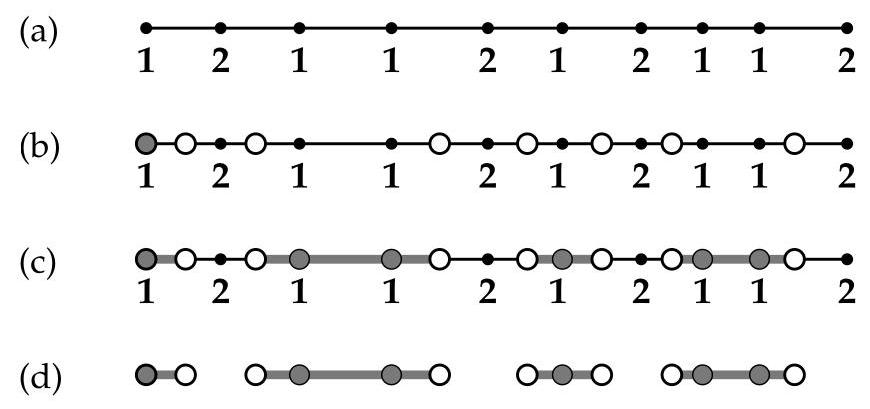
\includegraphics[width=0.6\textwidth]{images/ch07-fig09.jpg}
\caption{\({F}_{2}\) 的三角剖分， \({F}_{2}\) 是图\ref{fig:7.6}--\ref{fig:7.8}中三角形的底边，以线段作为子单纯形， \({\sum }_{2}\) 中的顶点(用小点标记)作为子极面。斯佩纳标号如(a)所示，与图\ref{fig:7.6}类似。 \({\sum }_{2}\) 的完全标记子单纯形在(b)中用白点标记，类似于图\ref{fig:7.7}中的黑点；完全标记的子极面是最左边用灰色标记的顶点，类似于图\ref{fig:7.7}中的任何一个白点。图 \({G}_{2}\) 如(c)所示，类似于图\ref{fig:7.8}，(d)中单独展示了该图，在这个维度中它只是一组路径。}
\label{fig:7.9}
\end{figure}
\bigskip

需要一种更系统的方法，为此我们考虑证明中命题(ii)从 \(n = 1\) 到 \(n = 2\) 的第一步归纳，如图\ref{fig:7.9}所示。极面 \({F}_{1}\) 仅由单个顶点 \({v}^{1}\) 组成，在左边标记为灰色节点。这定义了图 \({G}_{1}\) ，它没有边，但有一个由 \({v}^{1}\) 给出的节点(因此节点数为奇数)， \({v}^{1}\) 也是 \({\sum }_{1}\) 的唯一子单纯形且是完全标记的；图 \({G}_{1}\) 是唯一不由路径和环组成的图。在 \({\sum }_{2}\) 中，子单纯形是线段，它们的子极面是单个顶点。(\ref{eq:7.12})中的集合 \({C}^{\prime }\) 由那些标签为1的顶点组成，在图\ref{fig:7.9}中用灰色标记，此外最左边的灰色节点是 \(C\) 的唯一元素。这是 \({G}_{2}\) 中路径的一个端点。所有其他端点是 \({\sum }_{2}\) 中完全标记的子单纯形，如之前一样用白点标记。(因为 \({F}_{2}\) 只是一条线段，所以没有环。)

现在我们陈述斯佩纳引理的构造性版本，它是通过取所考虑图的并集得到的，该并集将它们的路径连接起来。

\bigskip
\noindent
\begin{proposition}\label{prop:7.11}
考虑单纯形 \(S\) 的三角剖分 \(\sum\) ，其顶点为 \({v}^{1},\ldots ,{v}^{d}\) ，并采用如定理\ref{theo:7.10}中的斯佩纳标号 \(d \geq  2\) 。设 \({G}_{1},\ldots ,{G}_{d}\) 是定理证明中定义的图，并按如下方式定义图 \(G\)

\begin{equation}
G = {G}_{1} \cup  \cdots  \cup  {G}_{d}\label{eq:7.13}
\end{equation}

其中并集分别对节点集和边集取。那么 \(G\) 中的每个节点的度数为1或2，因此 \(G\) 由路径和环组成。路径的端点由 \({v}^{1}\) 和 \(\sum\) 的完全标记子单纯形给出。
\end{proposition}

\bigskip
\noindent
\begin{proof}
设 \(1 \leq  n < d\) 。根据(\ref{eq:7.12})中的构造， \({G}_{n}\) 和 \({G}_{n + 1}\) 的公共节点是 \({\sum }_{n}\) 中具有 \(n\) 个顶点且所有顶点标签为 \(1,\ldots ,n\) 的子单纯形。对于 \(n > 1\) ，这些节点在 \({G}_{n}\) 和 \({G}_{n + 1}\) 中的度数均为1，因此在 \({G}_{n} \cup  {G}_{n + 1}\) 和 \(G\) 中的度数为2。因此，如所声称的， \(G\) 中度数为1的节点由 \({v}^{1}\) (它是 \({G}_{1}\) 中的唯一节点，在其中度数为0，在 \({G}_{2}\) 中度数为1)和 \({G}_{d}\) 中完全标记的子单纯形给出。
\end{proof}

\begin{figure}[htbp]
\centering
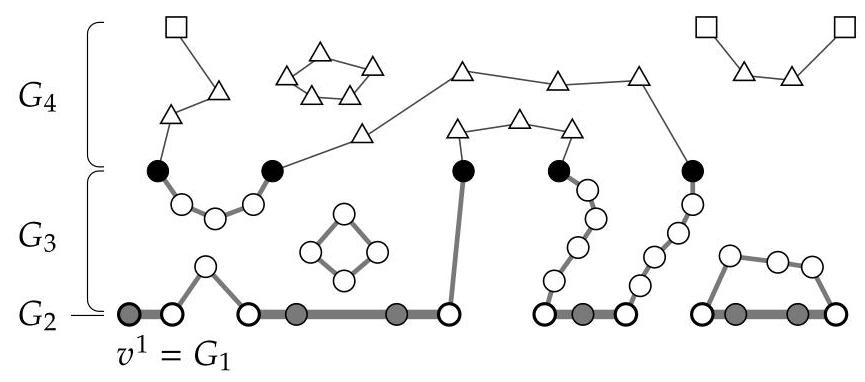
\includegraphics[width=0.6\textwidth]{images/ch07-fig10.jpg}
\caption{(\ref{eq:7.13})中 \(G\) 在 \(d = 4\) 情况下的示例。图 \({G}_{2}\) 取自图\ref{fig:7.9}。图\ref{fig:7.8}中的图 \({G}_{3}\) 被绘制为 \({\sum }_{2}\) 和 \({\sum }_{3}\) 的完全标记元素之间的一个“层”，图 \({G}_{4}\) 则作为另一个这样的层。三角形表示 \({\sum }_{4}\) 中标签为1、2、3的子极面(除黑点外，黑点也属于 \({G}_{3}\) )，正方形表示 \({\sum }_{4}\) 中标签为1、2、3、4的子单纯形。}
\label{fig:7.10}
\end{figure}

图\ref{fig:7.10}展示了 \(G\) 的一个示例，针对一个三角剖分的四面体，其底面极面是图\ref{fig:7.8}中的 \({F}_{3}\) 。来自 \({G}_{2},\ldots ,{G}_{d}\) 的拼接路径可能会形成新的循环，如右下角所示。从 \({v}^{1}\) 开始的路径终止于 \(\sum\) 中的一个完全标记子单纯形，因此通过沿着该路径可以找到它。该示例表明，路径可能会在不同维度间上下移动，例如访问 \({G}_{4}\) 中的一个三角形，然后回到 \({G}_{2}\) 中的一个顶点。(\ref{eq:7.13})中 \(G\) 的构造非常简洁，因为它不需要对三角剖分 \(\sum\) 及其标记顶点进行任何进一步的添加。

\section{KKM引理}\label{sec-7.5}

在本节中，我们使用斯佩纳引理来证明一个由克纳斯特(Knaster)、库拉托夫斯基(Kuratowski)和马祖尔克维奇(Mazurkiewicz)(1929年)提出的定理，该定理以作者姓氏首字母命名为“KKM引理”。KKM引理考虑一个单纯形 \(S\) ，其顶点为 \({v}^{1},\ldots ,{v}^{d}\) ，以及闭集 \({A}_{1},\ldots ,{A}_{d}\) 。与斯佩纳条件密切相关的假设是，对于任意顶点集， \(S\) 中以这些顶点 \({v}^{i}\) 构成的面被相应的闭集 \({A}_{i}\) 覆盖，如图\ref{fig:7.11}所示。结论是这些集合有一个公共点。在某些情况下，这样的闭集比试图寻找不动点的函数更自然地被定义，因此KKM引理本身就是一个有用的工具。无论如何，它几乎可以立即导出单位单纯形上布劳威尔不动点定理的证明(定理\ref{theo:7.13})。作为背景材料，我们回顾欧几里得范数与距离的概念，以及关于收敛子列存在性的经典波尔查诺 - 魏尔斯特拉斯定理，该定理用于KKM引理的证明。

背景材料:欧几里得范数与距离

对于 \(a = {\left( {a}_{1},\ldots ,{a}_{d}\right) }^{\top } \in  {\mathbb{R}}^{d}\) ， \(a\) 的欧几里得范数 \(\parallel a\parallel\) 定义为

\[
\parallel a\parallel  = \sqrt{{a}^{\top }a} = \sqrt{{a}_{1}^{2} + \cdots  + {a}_{d}^{2}}.
\]

两点 \(a,b \in  {\mathbb{R}}^{d}\) 之间的欧几里得距离定义为 \(\parallel a - b\parallel\) 。

\bigskip
\noindent
\begin{theorem}[KKM引理]\label{theo:7.12}
设 \(S\) 是一个顶点为 \({v}^{1},\ldots ,{v}^{d}\) 的单纯形，设 \({A}_{1},\ldots ,{A}_{d}\) 是闭集，使得对于所有 \(I \subseteq  \{ 1,\ldots ,d\}\) ， \(S\) 中以这些顶点构成的面 \({F}_{I} = \operatorname{conv}\left\{  {{v}^{i} \mid  i \in  I}\right\}\) 是相应闭集 \(\mathop{\bigcup }\limits_{{i \in  I}}{A}_{i}\) 的子集。那么 \(\mathop{\bigcap }\limits_{{i = 1}}^{d}{A}_{i} \neq  \varnothing\) 。
\end{theorem}

\bigskip
\noindent
\begin{proof}
设 \(\varepsilon  > 0\) ，并考虑 \(S\) 的一个三角剖分 \({\sum }_{\varepsilon }\) ，使得对于 \({\sum }_{\varepsilon }\) 中的任何子单纯形 \(T\) 和任何 \(x,y \in  T\)，我们有 \(\parallel x - y\parallel  \leq  \varepsilon\) ；我们将在第\ref{sec-7.7}节中证明，对于任何 \(\varepsilon  > 0\)，这样的 \(\varepsilon\) - 精细三角剖分是存在的。对于 \({\sum }_{\varepsilon }\) 中的任何顶点 \(x\)，设 \(I \subseteq  \{ 1,\ldots ,d\}\) {\color{red}是满足 \(x \in  {F}_{I}\) 的极小元素}。根据假设， \({F}_{I} \subseteq  \mathop{\bigcup }\limits_{{i \in  I}}{A}_{i}\) ，因此对于某个 \(i \in  I\) ，有 \(x \in  {A}_{i}\) ，我们选择 \(i\) 作为 \(x\) 的标签。根据构造，这是一个斯佩纳标号。根据斯佩纳引理(定理\ref{theo:7.10})， \({\sum }_{\varepsilon }\) 中存在一个完全标记的子单纯形，其顶点为 \({w}_{\varepsilon }^{1},\ldots ,{w}_{\varepsilon }^{d}\)，使得 \({w}_{\varepsilon }^{i}\) 具有标签 \(i\) ，因此对于 \(1 \leq  i \leq  d\)，它属于 \({A}_{i}\)。

\bigskip
\noindent
{\bf 背景材料:}每个有界序列都有一个收敛子序列

波尔查诺 - 魏尔斯特拉斯定理指出:设 \({x}^{\left( 1\right) },{x}^{\left( 2\right) },\ldots\) 是 \({\mathbb{R}}^{d}\) 中的一个有界点列，即存在某个 \(M\) ，使得对于所有的 \(n\) ，都有 \(\begin{Vmatrix}{x}^{\left( n\right) }\end{Vmatrix} \leq  M\) 。那么这个序列有一个收敛子序列。

这个重要的定理有一个很好的证明，我们在此回顾一下。我们首先考虑一个有界的实数序列 \({y}^{\left( 1\right) },{y}^{\left( 2\right) },\ldots\) ，其中对于所有的 \(n\) 都有 \(\left| {y}^{\left( n\right) }\right|  \leq  M\) 。我们证明这个序列有一个单调子序列 \({y}^{\left( {k}_{1}\right) },{y}^{\left( {k}_{2}\right) },\ldots\) ，即要么 \({y}^{\left( {k}_{1}\right) } \geq  {y}^{\left( {k}_{2}\right) } \geq  \cdots\) 成立，要么 \({y}^{\left( {k}_{1}\right) } \leq  {y}^{\left( {k}_{2}\right) } \leq  \cdots\) 成立。把实数 \({y}^{\left( 1\right) },{y}^{\left( 2\right) },\ldots\) 想象成“海边酒店”的高度。从每个高度为 \({y}^{\left( k\right) }\) 的酒店顶部，只要后续高度为 \({y}^{\left( k + 1\right) },{y}^{\left( k + 2\right) },\ldots\) 的酒店高度更低，你就可以看到它们之外的景色，如果这些酒店的高度都更低，你还能看到无穷远处的大海。换句话说，如果一家酒店属于集合 \(K = \left\{  {k \mid  {y}^{\left( k\right) } > {y}^{\left( j\right) }\text{,对于所有}j > k}\right\}\)，那么它就有“海景”(想必，这些都是非常昂贵的酒店)。如果 \(K\) 是无限集，那么我们按升序取 \(K\) 中的元素作为下标 \({k}_{1},{k}_{2},{k}_{3},\ldots\) ，从而得到我们的子序列 \({y}^{\left( {k}_{1}\right) },{y}^{\left( {k}_{2}\right) },{y}^{\left( {k}_{3}\right) },\ldots\) ，它显然是递减的。然而，如果 \(K\) 是有限集，其最大元素为 \(m\) (如果 \(K\) 为空集，则取 \(m = 0\) )，那么对于每个 \(k > m\) ，我们有 \(k \notin  K\) ，因此存在某个 \(j > k\) 使得 \({y}^{\left( k\right) } \leq  {y}^{\left( j\right) }\) 。从 \({k}_{1} = m + 1\) 对应的 \({y}^{\left( {k}_{1}\right) }\) 开始，我们令 \({k}_{2} > {k}_{1}\) 且 \({y}^{\left( {k}_{1}\right) } \leq  {y}^{\left( {k}_{2}\right) }\) 。然后找到另一个 \({k}_{3} > {k}_{2}\) 使得 \({y}^{\left( {k}_{2}\right) } \leq  {y}^{\left( {k}_{3}\right) }\) ，依此类推，这样就得到一个弱递增子序列 \({y}^{\left( {k}_{1}\right) } \leq  {y}^{\left( {k}_{2}\right) } \leq  {y}^{\left( {k}_{3}\right) } \leq  \cdots\) 。无论哪种情况，原序列都有一个单调子序列。

这个单调子序列 \({y}^{\left( {k}_{1}\right) },{y}^{\left( {k}_{2}\right) },\ldots\) 是有界的，因为原序列是有界的。很容易证明，如果该子序列是递减的，它收敛于其元素的下确界；如果它是弱递增的，则收敛于其上确界。这就证明了实数序列在 \({\mathbb{R}}^{1}\) 中的波尔查诺 - 魏尔施特拉斯定理(Bolzano - Weierstrass theorem)。

为了证明该定理对于 \(n = 1,2,3,\ldots\) 时 \({\mathbb{R}}^{d}\) 中的点列 \({x}^{\left( n\right) } = \left( {{x}_{1}^{\left( n\right) },\ldots ,{x}_{d}^{\left( n\right) }}\right)\) 成立，注意到这些点的 \(i = 1,\ldots ,d\) 对应的分量 \({x}_{i}^{\left( n\right) }\) 是有界的，因为 \(\left| {x}_{i}^{\left( n\right) }\right|  \leq  \begin{Vmatrix}{x}^{\left( n\right) }\end{Vmatrix} \leq  M\) 。首先，找出第一个分量 \({x}_{1}^{\left( 1\right) },{x}_{1}^{\left( 2\right) },{x}_{1}^{\left( 3\right) },\ldots\) 的一个收敛子列，设其极限为 \({z}_{1}\) 。为了方便表示，用这个子列替换原来的点列，此时该子列的第一个分量收敛。其次，找出一个子列，使得第二个分量 \({x}_{2}^{\left( 1\right) },{x}_{2}^{\left( 2\right) },{x}_{2}^{\left( 3\right) },\ldots\) 有极限 \({z}_{2}\) ，这样一来，第一个和第二个分量都收敛。按照这种方式继续下去，我们得到一个极限为 \(\left( {{z}_{1},{z}_{2},\ldots ,{z}_{d}}\right)\) 的子列，从而完成了证明。

考虑一个趋于 0 的正实数序列 \(\varepsilon \left( 1\right) ,\varepsilon \left( 2\right) ,\ldots\) (例如， \(\varepsilon \left( n\right)  = \frac{1}{n}\) )， \(S\) 的一个 \(\varepsilon \left( n\right)\) - 精细三角剖分 \({\sum }_{\varepsilon \left( n\right) }\) ，以及前面所考虑的单纯形 \(S\) 中标签为 1 的对应点列 \({w}_{\varepsilon \left( 1\right) }^{1},{w}_{\varepsilon \left( 2\right) }^{1},\ldots\) 。因为

\begin{figure}[htbp]
\centering
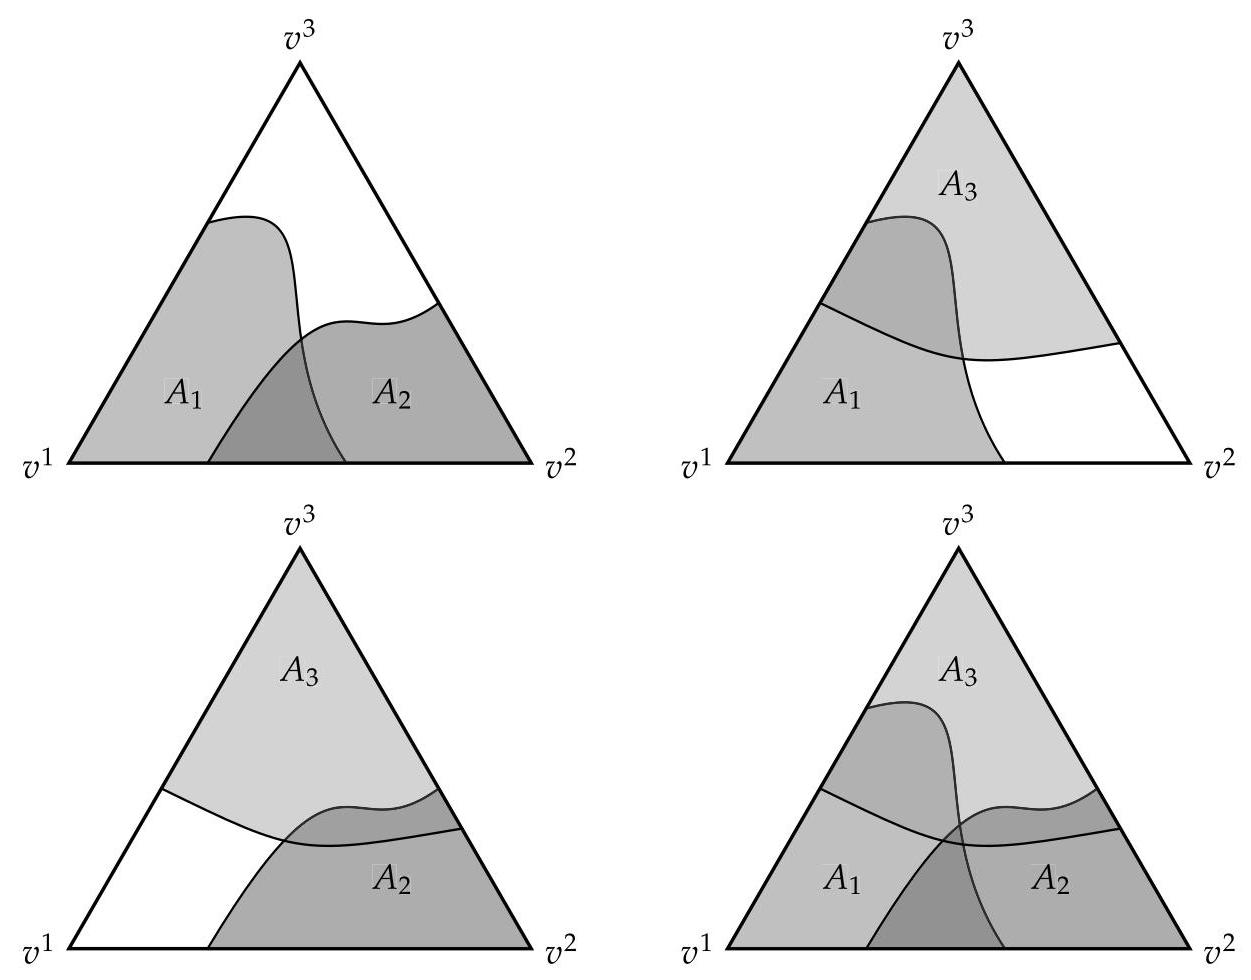
\includegraphics[width=0.9\textwidth]{images/ch07-fig11.jpg}
\caption{展示了对于 \(d = 3\) 、集合 \(I = \{ 1,2\} ,\{ 1,3\} ,\{ 2,3\}\) 和 \(\{ 1,2,3\}\) 的 KKM 引理的假设。}
\label{fig:7.11}
\end{figure}

由于 \(S\) 是有界闭集，这个点列有一个收敛子列，其极限 \(z\) 属于 \(S\) 。对于所有的 \(i = 1,\ldots ,d\) ，我们有 \(\begin{Vmatrix}{{w}_{\varepsilon \left( n\right) }^{1} - {w}_{\varepsilon \left( n\right) }^{i}}\end{Vmatrix} \leq  \varepsilon \left( n\right)\) ，使得该子列中标签为 \(i\) 的点 \({w}_{\varepsilon \left( n\right) }^{i}\) 当 \(n \rightarrow  \infty\) 时也收敛到 \(z\) ，其中 \({w}_{\varepsilon \left( n\right) }^{i} \in  {A}_{i}\) 。因为 \({A}_{i}\) 是闭集，所以 \(z \in  {A}_{i}\) 。因此，交集 \(\mathop{\bigcap }\limits_{{i = 1}}^{d}{A}_{i}\) 包含 \(z\) 且非空，正如所声称的那样。
\end{proof}

以下定理是将 KKM 引理应用于单位单纯形 \(\Delta\) 的直接结果。闭集 \({A}_{i}\) 是根据我们最初的定义(\ref{eq:7.2})在 \(\Delta\) 中标签为 \(i\) 的那些点 \(x\) 。


\bigskip
\noindent
\begin{theorem}[单位单纯形上的布劳威尔不动点定理]\label{theo:7.13}
式\eqref{eq:7.1}中 (d - 1) 维度的单位单纯形 \(\Delta\) 上的连续函数 \(f : \Delta  \rightarrow  \Delta\) 有一个不动点。
\end{theorem}

\bigskip
\noindent
\begin{proof}
对于 \(i = 1,\ldots ,d\) ，设 \({A}_{i} = \left\{  {x \in  \Delta  \mid  {x}_{i} \geq  {f}_{i}\left( x\right) }\right\}\) 。那么 \({A}_{i}\) 是一个闭集（回顾 \(f\) 的定义），因此 \({f}_{i}\) 是连续的。设 \(x \in  \Delta\) 且 \(I = \left\{  {i \mid  {x}_{i} > 0}\right\}\) 。因为 \(\Delta\) 的顶点是单位向量，定理\ref{theo:7.12}中的面 \({F}_{I}\) 是 \(\Delta\) 中包含 \(x\) 的最小极面。如引理\ref{lem:7.9}所示，存在某个 \(i\) 使得 \({x}_{i} > 0\) 且 \(x \in  {A}_{i}\) 。由于 \(x\) 是任意的，这表明对于任意 \(I \subseteq  \{ 1,\ldots ,d\}\) 有 \({F}_{I} \subseteq  \mathop{\bigcup }\limits_{{i \in  I}}{A}_{i}\) 。根据定理\ref{theo:7.12}，存在某个 \(z \in  \mathop{\bigcap }\limits_{{i = 1}}^{d}{A}_{i}\) ，根据引理\ref{lem:7.1}有 \(f\left( z\right)  = z\) 。
\end{proof}

\section{一般紧凸集上的布劳威尔不动点定理}\label{sec-7.6}

定理\ref{theo:7.13}表明单位单纯形 \(\Delta\) 上的连续函数有一个不动点。在本节中，我们证明对于某个 \({\mathbb{R}}^{k}\) 的子集——紧凸集 \(C\) 上的连续函数 \(f\) 也成立，这是布劳威尔不动点定理的一般形式。第一步是通过一个双射仿射映射将 \(C\) 嵌入到 \(\Delta\) 中。假设 \(C\) 是 \(\Delta\) 的一个子集，第二步是构造一个连续函数 \(p : \Delta  \rightarrow  C\) 使得对于 \(x \in  C\) 有 \(p\left( x\right)  = x\) 。那么由对于 \(x \in  \Delta\) 定义为 \(h\left( x\right)  = f\left( {p\left( x\right) }\right)\) 的连续函数 \(h : \Delta  \rightarrow  \Delta\) 有一个不动点，容易看出这个不动点也是给定函数 \(f : C \rightarrow  C\) 的不动点。

以下引理是关于将 \(C\) 嵌入到 \(\Delta\) 中的。

\bigskip
\noindent
\begin{lemma}\label{lem:7.14}
设 \(C \subset  {\mathbb{R}}^{k}\) ，且设 \(C\) 是一个维度为 \(d - 1\) 的紧凸集。那么存在一个从 \(C\) 到式\eqref{eq:7.1}中 (d - 1) 维度单位单纯形 \(\Delta\) 的单射仿射映射 \(J : C \rightarrow  \Delta\) 。
\end{lemma}

\bigskip
\noindent
\begin{proof}
因为 \(C\) 的维度为 \(d - 1\) ，所以它有 \(d\) 个(但不会更多)仿射无关的点 \({w}^{1},\ldots ,{w}^{d}\) 。如果 \(d = 1\) ，那么 \(C\) 只是一个点，因此我们可以假设 \(d > 1\) 。根据引理\ref{lem:7.2}，每个点 \(x \in  C\) 都是仿射组合 \(x = \mathop{\sum }\limits_{{i = 1}}^{d}{w}^{i}{\lambda }_{i}\) ，其中这个方程以及方程 \(\mathop{\sum }\limits_{{i = 1}}^{d}{\lambda }_{i} = 1\) 唯一地确定了系数 \({\lambda }_{1},\ldots ,{\lambda }_{d}\) 。因此，这些系数由一个从 \({\mathbb{R}}^{k}\) (包含 \(C\) )到 \({\mathbb{R}}^{d}\) 的线性映射定义，所以它们连续依赖于 \(x\) 。它们的最小值 \(\mathop{\min }\limits_{{1 \leq  i \leq  d}}{\lambda }_{i}\) 是 \(x\) 的连续函数，因此在紧集 \(C\) 上取得其最小值 \(M\) ，即

\begin{equation}
x = \mathop{\sum }\limits_{{i = 1}}^{d}{w}^{i}{\lambda }_{i},\;\mathop{\sum }\limits_{{i = 1}}^{d}{\lambda }_{i} = 1\; \Rightarrow  \;{\lambda }_{i} \geq  M\;\left( {x \in  C,1 \leq  i \leq  d}\right) .\label{eq:7.14}
\end{equation}

对于 \(x = {w}^{2}\) ，我们有 \({\lambda }_{1} = 0\) ，所以 \(M \leq  0\) 。设 \(w = \mathop{\sum }\limits_{{i = 1}}^{d}{w}^{i}\frac{1}{d}\) 为点 \({w}^{1},\ldots ,{w}^{d}\) 的重心。我们的目标是将点 \({w}^{i}\) “拉伸” 为新的点 \({v}^{i}\) (通常在 \(C\) 之外)，“远离 \({w}^{\prime \prime }\) ”，使得每个 \(x \in  C\) 是 \({v}^{1},\ldots ,{v}^{d}\) 的凸组合，而不仅仅是仿射组合。对于某个有待确定的 \(\alpha  > 0\) ，设

\[
{v}^{i} = w + \left( {{w}^{i} - w}\right) \alpha \;\left( {1 \leq  i \leq  d}\right)
\]

因此

\[
{w}^{i} = w + \left( {{v}^{i} - w}\right) \frac{1}{\alpha } = w\left( {1 - \frac{1}{\alpha }}\right)  + {v}^{i}\frac{1}{\alpha }.
\]

那么 \(w\) 也是点 \({v}^{1},\ldots ,{v}^{d}\) 的重心，因为

\[
\mathop{\sum }\limits_{{i = 1}}^{d}{v}^{i}\frac{1}{d} = \mathop{\sum }\limits_{{i = 1}}^{d}\left( {w + \left( {{w}^{i} - w}\right) \alpha }\right) \frac{1}{d} = w.
\]

因此，对于 \(x \in  C\) ，我们有

\begin{equation}
x = \mathop{\sum }\limits_{{i = 1}}^{d}{w}^{i}{\lambda }_{i} = \mathop{\sum }\limits_{{i = 1}}^{d}\left( {w\left( {1 - \frac{1}{\alpha }}\right)  + {v}^{i}\frac{1}{\alpha }}\right) {\lambda }_{i} = \mathop{\sum }\limits_{{i = 1}}^{d}{v}_{i}\left( {\frac{1}{d}\left( {1 - \frac{1}{\alpha }}\right)  + {\lambda }_{i}\frac{1}{\alpha }}\right)\label{eq:7.15}
\end{equation}

其中我们希望对于 \(1 \leq  i \leq  d\) 能满足

\begin{equation}
\frac{1}{d}\left( {1 - \frac{1}{\alpha }}\right)  + {\lambda }_{i}\frac{1}{\alpha } \geq  0\label{eq:7.16}
\end{equation}

如果 \({\lambda }_{i} \geq  \frac{1 - \alpha }{d}\) 成立，那么该式成立，并且由于(\ref{eq:7.14})，如果 \(M \geq  \frac{1 - \alpha }{d}\) 成立则该式也成立。为此，选择 \(\alpha  = 1 - {Md}\) 就足够了(注意 \(M \leq  0\) )。此外， \(\mathop{\sum }\limits_{{i = 1}}^{d}\left( {\frac{1}{d}\left( {1 - \frac{1}{\alpha }}\right)  + {\lambda }_{i}\frac{1}{\alpha }}\right)  = 1\) ，所以(\ref{eq:7.16})和(\ref{eq:7.15})意味着 \(C\) 是顶点为 \({v}^{1},\ldots ,{v}^{d}\) 的单纯形 \(T\) 的子集。根据引理\ref{lem:7.3}，存在一个仿射双射 \(T \rightarrow  \Delta\) ，它在 \(C\) 上的限制给出了所需的仿射单射 \(J : C \rightarrow  \Delta\) 。
\end{proof}
\bigskip

设 \(C\) 是一个紧凸集，设 \(D = J\left( C\right)\) 是 \(C\) 在引理\ref{lem:7.14}中的仿射单射 \(J\) 下的像。集合 \(D\) 是 \(\Delta\) 的一个闭凸子集。接下来，我们构造一个连续函数 \(p : \Delta  \rightarrow  D\) ，它在 \(D\) 上的限制是恒等映射，即对于 \(x \in  D\) 有 \(p\left( x\right)  = x\) 。下面的函数 \(p\) 是最容易使用的。

设 \(D\) 为 \({\mathbb{R}}^{d}\) 的任意非空闭凸子集。到 \(D\) 上的投影是为 \(x \in  {\mathbb{R}}^{d}\) 定义的函数 \(p : {\mathbb{R}}^{d} \rightarrow  D\) ，其定义如下

\begin{equation}
p\left( x\right)  = \arg \mathop{\min }\limits_{{z \in  D}}\parallel x - z\parallel .\label{eq:7.17}
\end{equation}

条件 (\ref{eq:7.17}) 意味着 \(p\left( x\right)\) 是 \(D\) 中与 \(x\) 的欧几里得距离最近的点 \(z\) ，显然，如果 \(x \in  D\) ，则 \(p\left( x\right)  = x\) 。因为 \(D\) 是非空且闭的，并且距离有下界零，所以 \(D\) 中存在这样一个最近的点。我们很快会看到这个点也是唯一的，因此 \(p\left( x\right)\) 是良定义的。然后我们将证明 \(p\) 是一个连续函数。我们首先需要一些欧几里得范数的性质。

如果 \({a}^{\top }b = 0\) ，则称一般向量 \(a,b \in  {\mathbb{R}}^{d}\) 是正交的 (orthogonal)。(这包括 \(a\) 或 \(b\) 是零向量的情况，在以下的讨论中通常会以某种平凡的方式涵盖这种情况。)那么，以 \(a,\mathbf{0},b\) 为顶点的三角形在 0 处有一个直角，勾股定理适用

\[
{a}^{\top }b = 0\; \Leftrightarrow  \;\parallel a - b{\parallel }^{2} = \parallel a{\parallel }^{2} + \parallel b{\parallel }^{2},
\]

\begin{center}
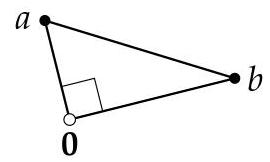
\includegraphics[width=0.2\textwidth]{images/ch07-fig12.jpg}
\end{center}
\hspace*{3em} 

这是因为对于任意 \(a,b\) ，我们有 \({b}^{\top }a = {a}^{\top }b \in  \mathbb{R}\) 且

\begin{equation}
\parallel a - b{\parallel }^{2} = {\left( a - b\right) }^{\top }\left( {a - b}\right)  = {a}^{\top }a - {a}^{\top }b - {b}^{\top }a + {b}^{\top }b = \parallel a{\parallel }^{2} - 2{a}^{\top }b + \parallel b{\parallel }^{2}.\label{eq:7.18}
\end{equation}

因此，

\begin{equation}
{a}^{\top }b = 0\; \Rightarrow  \;\parallel a - b\parallel  \geq  \parallel a\parallel ,\;\parallel a - b\parallel  \geq  \parallel b\parallel .\label{eq:7.19}
\end{equation}

以下引理涉及点 \(x\) 到由端点 \(c\) 经过另一点 \(b\) 所确定的射线 上的点的距离，该射线由集合 \(\{ c + \left( {b - c}\right) \lambda  \mid  \lambda  \geq  0\}\) 给出。如图\ref{fig:7.12} 所示，这取决于 \({\left( x - c\right) }^{\top }\left( {b - c}\right)\) 的符号，它表示向量 \(x - c\) 和 \(b - c\) 之间的角 (angle)；如果 \({\left( x - c\right) }^{\top }\left( {b - c}\right)  > 0\) ，则该角为锐角；如果 \({\left( x - c\right) }^{\top }\left( {b - c}\right)  < 0\) ，则为钝角；如果 \({\left( x - c\right) }^{\top }\left( {b - c}\right)  = 0\) ，则为直角。恰好在后两种情况下，射线上距离 \(x\) 最近的点是其端点 \(c\) 。

\begin{figure}[htbp]
\centering
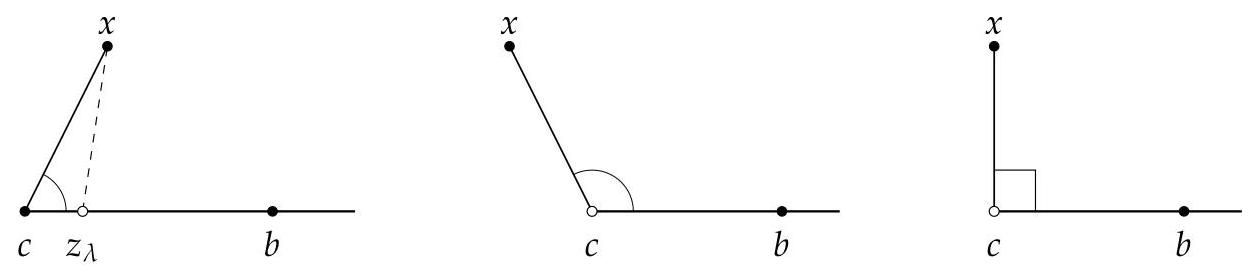
\includegraphics[width=0.9\textwidth]{images/ch07-fig13.jpg}
\caption{引理\ref{lem:7.15} (a)(左)和 (b)(中、右)的图示。}
\label{fig:7.12}
\end{figure}

\bigskip
\noindent
\begin{lemma}\label{lem:7.15}
设 \(x,b,c \in  {\mathbb{R}}^{d}\) 满足 \(b \neq  c\) ，且对于 \(\lambda  \in  \mathbb{R}\) 有 \({z}_{\lambda } = c + \left( {b - c}\right) \lambda\) 。则

(a) 对于所有足够小的正的 \(\lambda\) ，有 \({\left( x - c\right) }^{\top }\left( {b - c}\right)  \leq  0 \Leftrightarrow  \begin{Vmatrix}{x - {z}_{\lambda }}\end{Vmatrix} > \parallel x - c\parallel\) 。

(b) 对于所有 \(\lambda  > 0\) ，有 \({\left( x - c\right) }^{\top }\left( {b - c}\right)  \leq  0 \Leftrightarrow  \begin{Vmatrix}{x - {z}_{\lambda }}\end{Vmatrix} > \parallel x - c\parallel\) 。
\end{lemma}

\bigskip
\noindent
\begin{proof}
由 (\ref{eq:7.18})，

\[
{\begin{Vmatrix}x - {z}_{\lambda }\end{Vmatrix}}^{2} = {\left( x - {z}_{\lambda }\right) }^{\top }\left( {x - {z}_{\lambda }}\right)
\]

\[
= {\left( x - c - \left( b - c\right) \lambda \right) }^{\top }\left( {x - c - \left( {b - c}\right) \lambda }\right)
\]

\[
= \parallel x - c{\parallel }^{2} - 2{\left( x - c\right) }^{\top }\left( {b - c}\right) \lambda  + \parallel b - c{\parallel }^{2}{\lambda }^{2}
\]

\[
= \parallel x - c{\parallel }^{2} - \left( {2{\left( x - c\right) }^{\top }\left( {b - c}\right)  - \parallel b - c{\parallel }^{2}\lambda }\right) \lambda .
\]

因此，如果 \({\left( x - c\right) }^{\top }\left( {b - c}\right)  > 0\) ，那么对于足够小的正 \(\lambda\) 有 \(\begin{Vmatrix}{x - {z}_{\lambda }}\end{Vmatrix} < \parallel x - c\parallel\) ；如果 \({\left( x - c\right) }^{\top }\left( {b - c}\right)  \leq  0\) ，那么对于所有 \(\lambda  > 0\) 有 \(\begin{Vmatrix}{x - {z}_{\lambda }}\end{Vmatrix} > \parallel x - c\parallel\) 。这表明了 (a) 和 (b) 中的 “ \(\Rightarrow\) ”。为了证明 (a) 中的反向蕴含关系 “ \(\Leftarrow\) ”，对于某个 \(\lambda  > 0\) 有 \(\begin{Vmatrix}{x - {z}_{\lambda }}\end{Vmatrix} < \parallel x - c\parallel\) 且 \({\left( x - c\right) }^{\top }\left( {b - c}\right)  \leq  0\) 会与 (b) 中的 “ \(\Rightarrow\) ” 矛盾。类似地，(b) 中的 “ \(\Leftarrow\) ” 成立，因为对于某个足够小的 \(\lambda  > 0\) 有 \(\begin{Vmatrix}{x - {z}_{\lambda }}\end{Vmatrix} > \parallel x - c\parallel\) 且 \({\left( x - c\right) }^{\top }\left( {b - c}\right)  > 0\) 与 (a) 中的 “ \(\Rightarrow\) ” 矛盾。
\end{proof}
\bigskip

引理\ref{lem:7.15} 表明，对于非空闭凸集 \(D\) ， \(D\) 中距离 \(x\) 最近的点 \(c\) 是唯一的，因此 (\ref{eq:7.17}) 中的 \(p\left( x\right)  = c\) 是良定义的:即，如果 \(b\) 是 \(D\) 中的任意其他点且 \({\left( x - c\right) }^{\top }\left( {b - c}\right)  > 0\) ，那么根据引理\ref{lem:7.15}(a)，存在一个点 \({z}_{\lambda }\) ，它比 \(c\) 更接近 \(x\) ，其中对于 \(0 < \lambda  \leq  1\) ，这个点属于 \(D\) ，因为 \(D\) 是凸集，所以 \(c\) 不是 \(D\) 中距离 \(x\) 最近的点，这是一个矛盾；如果 \({\left( x - c\right) }^{\top }\left( {b - c}\right)  \leq  0\) ，那么结合 \(\lambda  = 1\) (从而 \({z}_{\lambda } = b\) )应用引理\ref{lem:7.15}(b) 表明， \(b\) 到 \(x\) 的距离 \(\parallel x - b\parallel\) 比 \(c\) 到 \(x\) 的距离更大。此外，我们已经证明了以下内容。

\bigskip
\noindent
\begin{corollary}\label{cor:7.16}
设 \(D\) 是 \({\mathbb{R}}^{d}\) 的非空闭凸子集， \(x \in  {\mathbb{R}}^{d}\) ，并且设 \(c = p\left( x\right)\) 是 \(x\) 在 \(D\) 上的投影。那么对于所有 \(b \in  D\) 有 \({\left( x - c\right) }^{\top }\left( {b - c}\right)  \leq  0\) 。
\end{corollary}

\begin{figure}[htbp]
\centering
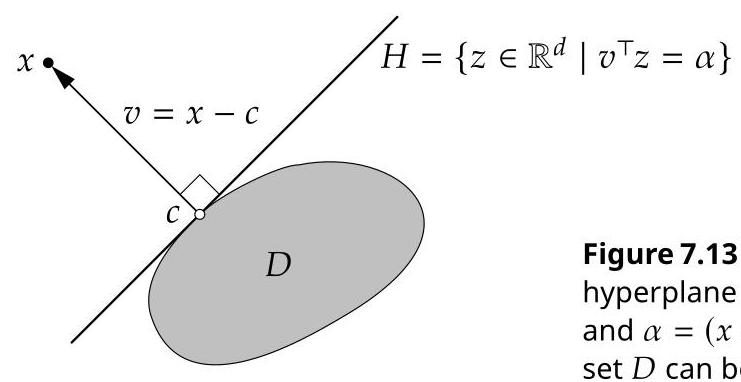
\includegraphics[width=0.5\textwidth]{images/ch07-fig14.jpg}
\caption{对于推论\ref{cor:7.16} 中的 \(x \notin D\) ，具有法向量 \(v = x - c\) 且 \(\alpha = {\left( x - c\right) }^{\top }c\) 的超平面 \(H\) 将 \(x\) 与 \(D\) 分隔开。(集合 \(D\) 可以是无界的。)}
\label{fig:7.13}
\end{figure}


推论\ref{cor:7.16}也被称为分离超平面定理。在 \({\mathbb{R}}^{d}\) 中的一个超平面 \(H\) 定义为 \(H = \left\{  {z \in  {\mathbb{R}}^{d} \mid  {v}^{\top }z = \alpha }\right\}\) ，其中 \(v\) 是 \({\mathbb{R}}^{d}\) 中的非零法向量， \(\alpha\) 是实数。相应的半空间定义为 \(\left\{  {z \in  {\mathbb{R}}^{d} \mid  {v}^{\top }z \leq  \alpha }\right\}\) 。假设在推论\ref{cor:7.16}中我们有 \(x \notin  D\) ，因此 \(x \neq  c\) 和 \({\left( x - c\right) }^{\top }\left( {x - c}\right)  = \parallel x - c{\parallel }^{2} > 0\) 。对于 \(v = x - c\) 和 \(\alpha  = {\left( x - c\right) }^{\top }c\) ，该推论表明 \(D\) 是由 \(H\) 定义的半空间的一个子集，而 \(x\) 显然不在这个半空间中，因此被 \(H\) 从 \(D\) 中“分离”出来。另见 图\ref{fig:7.13}。分离超平面定理是一个非常有用的工具，但必须确保其假设成立，特别是集合 \(D\) 是闭集。

引理\ref{lem:7.15}的第二个简单推论是，点 \(x\) 到直线 \(L\) 的最短连接线段与该直线正交。

\begin{center}
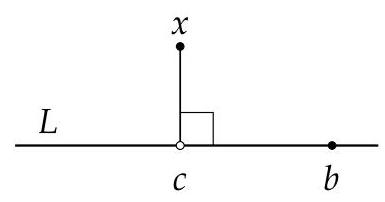
\includegraphics[width=0.3\textwidth]{images/ch07-fig15.jpg}
\end{center}
\hspace*{3em} 

\bigskip
\noindent
\begin{lemma}\label{lem:7.17}
设 \(L\) 是 \({\mathbb{R}}^{d}\) 中的一条直线，即 \({\mathbb{R}}^{d}\) 中两个点的仿射组合的集合，设 \(x \in  {\mathbb{R}}^{d}\) ，并设 \(c = p\left( x\right)\) 是 \(x\) 在 \(L\) 上的投影。那么对于所有 \(b \in  L\) 有 \({\left( x - c\right) }^{\top }\left( {b - c}\right)  = 0\) 。
\end{lemma}

\bigskip
\noindent
\begin{proof}
设 \(b\) 是 \(L\) 上除 \(c\) 之外的任意一点。那么 \(L = \{ c + \left( {b - c}\right) \lambda  \mid  \lambda  \in  \mathbb{R}\}\) 。如果 \({\left( x - c\right) }^{\top }\left( {b - c}\right)  > 0\) ，那么根据引理\ref{lem:7.15}(a)， \(c\) 不是到 \(x\) 的最近点。如果 \({\left( x - c\right) }^{\top }\left( {b - c}\right)  < 0\) ，设 \({b}^{\prime } = c + \left( {b - c}\right) \left( {-1}\right)\) 使得 \({b}^{\prime } - c =  - \left( {b - c}\right)\) ，并将 \(b\) 替换为 \({b}^{\prime }\) 来观察同样的情况，同样根据引理\ref{lem:7.15}(a)。因此，如所声称的那样有 \({\left( x - c\right) }^{\top }\left( {b - c}\right)  = 0\) 。
\end{proof}

我们的目标是证明(\ref{eq:7.17})中的投影映射 \(p\) 是连续的。这是以下定理的一个推论。

\bigskip
\noindent
\begin{theorem}\label{theo:7.18}
设 \(D\) 是 \({\mathbb{R}}^{d}\) 的一个非空闭凸子集，并设 \(p : {\mathbb{R}}^{d} \rightarrow  D\) 是(\ref{eq:7.17})中定义的到 \(D\) 上的投影。那么对于所有 \(x,y \in  {\mathbb{R}}^{d}\)

\begin{equation}
\parallel p\left( x\right)  - p\left( y\right) \parallel  \leq  \parallel x - y\parallel .\label{eq:7.20}
\end{equation}
\end{theorem}

\begin{figure}[htbp]
\centering
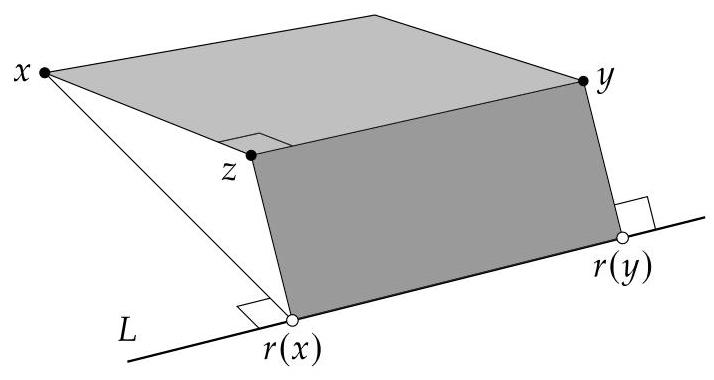
\includegraphics[width=0.5\textwidth]{images/ch07-fig16.jpg}
\caption{到直线 \(L\) 上的投影 \(r\left( x\right)\) 和 \(r\left( y\right)\) 。}
\label{fig:7.14}
\end{figure}

\bigskip
\noindent
\begin{proof}
设 \(x,y \in  {\mathbb{R}}^{d}\) 。我们首先证明当 \(D\) 是一条直线 \(L\) 时的结论，即

\begin{equation}
\parallel r\left( x\right)  - r\left( y\right) \parallel  \leq  \parallel x - y\parallel\label{eq:7.21}
\end{equation}

其中 \(r\left( x\right)\) 和 \(r\left( y\right)\) 分别表示 \(x\) 和 \(y\) 在 \(L\) 上的投影。这一结论从图\ref{fig:7.14}中显而易见，在图中我们考虑点 \(z = r\left( x\right)  + y - r\left( y\right)\) ，使得点 \(z,y,r\left( y\right) ,r\left( x\right)\) 构成一个矩形，其中 \(\parallel z - y\parallel  = \parallel r\left( x\right)  - r\left( y\right) \parallel\) ，并且点 \(x,z,y\) 是一个矩形的三个顶点，其边长 \(\parallel z - y\parallel\) 不大于对角线长度 \(\parallel x - y\parallel\) 。形式上，

\[
{\left( x - z\right) }^{\top }\left( {y - z}\right)
\]

\[
= {\left( x - r\left( x\right)  - y + r\left( y\right) \right) }^{\top }\left( {r\left( y\right)  - r\left( x\right) }\right)
\]

\[
= {\left( x - r\left( x\right) \right) }^{\top }\left( {r\left( y\right)  - r\left( x\right) }\right)  - {\left( y - r\left( y\right) \right) }^{\top }\left( {r\left( x\right)  - r\left( y\right) }\right)
\]

\[
= 0 - 0
\]

这里我们两次使用引理\ref{lem:7.17}，其中 \(r\left( x\right)\) 是 \(L\) 上距离 \(x\) 最近的点， \(r\left( y\right)\) 是 \(L\) 上距离 \(y\) 最近的点。那么(\ref{eq:7.19})式意味着 \(\parallel x - y\parallel  = \parallel x - z - \left( {y - z}\right) \parallel  \geq\)  \(\parallel y - z\parallel  = \parallel y - \left( {r\left( x\right)  + y - r\left( y\right) }\right) \parallel  = \parallel r\left( y\right)  - r\left( x\right) \parallel  = \parallel r\left( x\right)  - r\left( y\right) \parallel\) ，这就证明了(\ref{eq:7.21})式。

\begin{figure}[htbp]
\centering
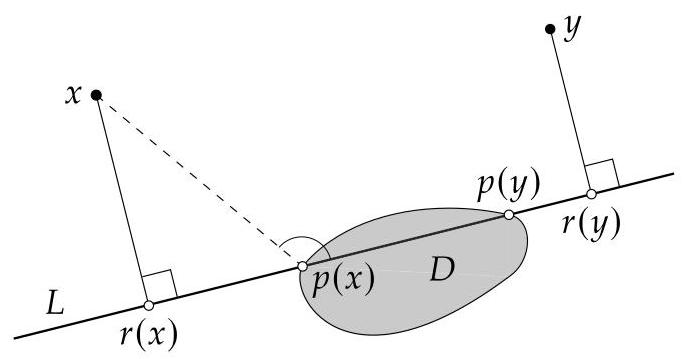
\includegraphics[width=0.5\textwidth]{images/ch07-fig17.jpg}
\caption{\(x\) 和 \(y\) 在凸集 \(D\) 上的投影 \(p\left( x\right)\) 和 \(p\left( y\right)\) ，以及过 \(p\left( x\right)\) 和 \(p\left( y\right)\) 的直线 \(L\) 。 \(x,p\left( x\right)\) 与 \(p\left( y\right)\) 之间的角不可能是锐角，所以 \(r\left( x\right)\) 在 \(p\left( x\right)\) 的左侧(或与之重合)。类似地， \(r\left( y\right)\) 在 \(p\left( y\right)\) 的右侧(或与之重合)。}
\label{fig:7.15}
\end{figure}


其次，现在考虑一个一般的非空闭凸集 \(D\) ，图\ref{fig:7.15}给出了二维情形下的一个示例。设 \(p\left( x\right)\) 和 \(p\left( y\right)\) 分别是 \(x\) 和 \(y\) 在 \(D\) 上的投影，这里我们可以假设 \(p\left( x\right)  \neq  p\left( y\right)\) ，因为否则(\ref{eq:7.20})式显然成立。设 \(L\) 是过 \(p\left( x\right)\) 和 \(p\left( y\right)\) 的直线，设 \(r\left( x\right)\) 和 \(r\left( y\right)\) 分别是 \(x\) 和 \(y\) 在 \(L\) 上的投影。

连接 \(p\left( x\right)\) 和 \(p\left( y\right)\) 的线段是 \(D\) 的子集，因为 \(D\) 是凸集。我们证明它是连接 \(r\left( x\right)\) 和 \(r\left( y\right)\) 的线段的子集，因此长度至多相同。设 \(c = p\left( x\right)\) 且 \(b = p\left( y\right)\) 。根据推论\ref{cor:7.16}， \({\left( x - c\right) }^{\top }\left( {b - c}\right)  \leq  0\) ，即图\ref{fig:7.15}中 \(c\) 处的角是直角或钝角。设 \(r\left( x\right)  = p\left( x\right)  + \left( {p\left( y\right)  - p\left( x\right) }\right) \lambda  = {z}_{\lambda }\) 。那么 \(\lambda  \leq  0\) ，因为如果 \(\lambda  > 0\) ，则引理\ref{lem:7.15}(b)将意味着 \(\parallel x - r\left( x\right) \parallel  > \parallel x - p\left( x\right) \parallel\) ，这是矛盾的，因为 \(p\left( x\right)  \in  L\) 且 \(r\left( x\right)\) 是 \(L\) 上距离 \(x\) 最近的点。类似地， \(r\left( y\right)  = p\left( y\right)  + \left( {p\left( x\right)  - p\left( y\right) }\right) \mu\) ，其中 \(\mu  \leq  0\) 。那么

\[
\parallel r\left( x\right)  - r\left( y\right) \parallel  = \parallel p\left( x\right)  + \left( {p\left( y\right)  - p\left( x\right) }\right) \lambda  - p\left( y\right)  - \left( {p\left( x\right)  - p\left( y\right) }\right) \mu \parallel
\]

\[
= \parallel \left( {p\left( x\right)  - p\left( y\right) }\right) \left( {1 - \lambda  - \mu }\right) \parallel
\]

\[
= \begin{Vmatrix}\left( {p\left( x\right)  - p\left( y\right) }\right) \end{Vmatrix}\left( {1 - \lambda  - \mu }\right)
\]

\[
\geq  \parallel \left( {p\left( x\right)  - p\left( y\right) }\right) \parallel
\]

因为 \(\lambda  \leq  0\) 和 \(\mu  \leq  0\) ，结合(\ref{eq:7.21})可推出(\ref{eq:7.20})。
\end{proof}
\bigskip

定理\ref{theo:7.18}表明，到 \(p\) 上的投影 \(D\) 是“压缩的”，因此确实是连续的:

\bigskip
\noindent
\begin{corollary}\label{cor:7.19}
设 \(D\) 是 \({\mathbb{R}}^{d}\) 的一个非空闭凸子集。那么，(\ref{eq:7.17}) 中从 \({\mathbb{R}}^{d}\) 到 \(D\) 的投影映射 \(p\) 是连续的。
\end{corollary}

\bigskip
\noindent
\begin{proof}
\(p : {\mathbb{R}}^{d} \rightarrow  D\) 的连续性意味着对于所有 \(x,y \in  {\mathbb{R}}^{d}\)

\[
\forall \varepsilon  > 0\exists \delta  > 0 : \parallel x - y\parallel  < \delta  \Rightarrow  \parallel p\left( x\right)  - p\left( y\right) \parallel  < \varepsilon .
\]

根据定理\ref{theo:7.18}，取 \(\delta  = \varepsilon\) 就足够了。
\end{proof}

推论\ref{cor:7.19}中集合 \(D\) 的凸性是至关重要的。例如，如果 \(D\) 只是由两个不同的点 \(a\) 和 \(b\) 组成的集合，那么对于与 \(a\) 和 \(b\) 等距的点，到 \(D\) 上的投影 \(p\) 是没有明确定义的，并且无论如何，在这些点附近会从 \(a\) “跳跃”到 \(b\) 。此外，交换 \(a\) 和 \(b\) 的函数 \(D \rightarrow  D\) 显然是连续的，但没有不动点。根据以下定理的证明，如果 \(p\) 是连续的，它应该有不动点。这个定理就是一般形式的布劳威尔不动点定理。

\bigskip
\noindent
\begin{theorem}\label{theo:7.20}
设 \(C\) 是 \({\mathbb{R}}^{k}\) 的一个非空紧凸子集，并且 \(f : C \rightarrow  C\) 是连续的。那么 \(f\) 有一个不动点 \(z \in  C\) ，即 \(f\left( z\right)  = z\) 。
\end{theorem}

\bigskip
\noindent
\begin{proof}
假设 \(C\) 的维度为 \(d - 1\) 。根据引理\ref{lem:7.14}，存在一个仿射单射 \(J : C \rightarrow  \Delta\) ，其像为 \(D = J\left( C\right)  = \{ J\left( z\right)  \mid  z \in  C\}  \subseteq  \Delta\) ，并且它的反函数 \({J}^{-1} : D \rightarrow  C\) 是一个线性双射。集合 \(D\) 是紧的，并且是凸的，因为 \(J\) 保持凸组合。定义函数 \(g : D \rightarrow  D\) 为

\begin{equation}
g\left( {J\left( z\right) }\right)  = J\left( {f\left( z\right) }\right) ,\label{eq:7.22}
\end{equation}

这是明确的，因为 \(J\) 是单射，并且由于 \(D = J\left( C\right)\) ，它在整个 \(D\) 上定义了 \(g\) 。那么对于所有 \(z \in  C\)

\begin{equation}
f\left( z\right)  = z\; \Leftrightarrow  \;g\left( {J\left( z\right) }\right)  = J\left( z\right)\label{eq:7.23}
\end{equation}

其中“ \(\Rightarrow\) ” 直接由 (\ref{eq:7.22}) 得出，而 “ \(\Leftarrow\) ” 成立是因为 \(g\left( {J\left( z\right) }\right)  = J\left( z\right)\) 意味着

\[
f\left( z\right)  = {J}^{-1}\left( {J\left( {f\left( z\right) }\right) }\right)  = {J}^{-1}\left( {g\left( {J\left( z\right) }\right) }\right)  = {J}^{-1}\left( {J\left( z\right) }\right)  = z.
\]

条件 (\ref{eq:7.23}) 表明， \(f\) 的不动点通过双射 \(J\) 与 \(g\) 的不动点一一对应。

设 \(p : \Delta  \rightarrow  D\) 是如 (\ref{eq:7.17}) 中所定义的到 \(D\) 上的投影映射，根据推论\ref{cor:7.19}，它是连续的，并且对于所有 \(x \in  D\) 满足 \(p\left( x\right)  = x\) 。定义函数

\[
h : \Delta  \rightarrow  \Delta ,\;h\left( x\right)  = g\left( {p\left( x\right) }\right) \;\left( {x \in  \Delta }\right) ,
\]

这是单位单纯形 \(\Delta\) 上的一个连续函数，因为 \(p\) 和 \(g\) 是连续的。根据定理\ref{theo:7.13}， \(h\) 有一个不动点 \(x \in  \Delta\) ，即 \(h\left( x\right)  = g\left( {p\left( x\right) }\right)  = x\) ，其中 \(h\left( x\right)  \in  D\) 是因为 \(g\) 只在 \(D\) 中取值，因此 \(p\left( x\right)  = x\) ，这意味着 \(g\left( x\right)  = x\) 。也就是说， \(h\) 的不动点恰好是 \(g\) 的不动点。根据 (\ref{eq:7.23})， \(f\) 的所需不动点由 \(z = {J}^{-1}\left( x\right)\) 给出。
\end{proof}

\section{弗赖登塔尔三角剖分}\label{sec-7.7}

本节补充了布劳威尔不动点定理证明中缺失的部分，即单纯形的任意精细三角剖分，该三角剖分用于证明KKM引理(定理\ref{theo:7.12})。如第\ref{sec-7.3}节末尾所述，仅当单纯形的维度为一维或二维时，这一点才显而易见。下面我们将介绍一种由弗赖登塔尔(Freudenthal，1942)提出的精妙三角剖分方法，该方法适用于任意维度。其构造基于两个主要思想:

\begin{itemize}
\item \(d\) 维单位立方体
\end{itemize}

\[
{C}_{d} = {\left\lbrack  0,1\right\rbrack  }^{d} = \left\{  {x \in  {\mathbb{R}}^{d} \mid  0 \leq  {x}_{i} \leq  1,1 \leq  i \leq  d}\right\}
\]

可以很容易地细分为小“立方体块”。

\begin{itemize}
\item 立方体 \({C}_{d}\) 有一个规范的三角剖分，可将其划分为 \(d\) ! 个单纯形，同样的方法也可应用于这些立方体块，从而得到 \({C}_{d}\) 三角剖分中某个单纯形的三角剖分。
\end{itemize}

我们继续用 \(d\) 表示所考虑点所在空间 \({\mathbb{R}}^{d}\) 的维度。式\eqref{eq:7.1}中的单位单纯形 \(\Delta\) 是 \({\mathbb{R}}^{d}\) 的一个子集，但其维度为 \(d - 1\) 。对于弗赖登塔尔三角剖分，我们使用一个比 \(\Delta\) 对称性更低的单纯形 \({T}_{d}\) ，这并不影响结果，因为根据引理\ref{lem:7.3}，给定维度的任意两个单纯形通过它们的重心坐标存在仿射双射。单纯形 \({T}_{d}\) 在 \({\mathbb{R}}^{d}\) 中有 \(d + 1\) 个顶点，因此其维度为 \(d\) ，根据引理\ref{lem:7.2}，这是最大维度。(具有此性质的有界多面体也称为满维多面体。)

单纯形 \({T}_{d}\) 是单位立方体 \({C}_{d}\) 某些顶点的凸包。例如，如果 \(d = 3\) ，那么 \({T}_{d}\) 是向量的凸包

\begin{equation}
\left( \begin{array}{l} 0 \\  0 \\  0 \end{array}\right) ,\left( \begin{array}{l} 1 \\  0 \\  0 \end{array}\right) ,\left( \begin{array}{l} 1 \\  1 \\  0 \end{array}\right) ,\left( \begin{array}{l} 1 \\  1 \\  1 \end{array}\right)\label{eq:7.24}
\end{equation}

这些向量中的第一个是 \({\mathbb{R}}^{d}\) 中的0向量，后续向量总是通过将一个分量从0变为1得到，最后一个向量是 \({\mathbb{R}}^{d}\) 中的全1向量1。然后我们从两个方面对 \({T}_{d}\) 进行推广:

(a) 分量从0变为1的不同顺序会生成 \(d\) ! 个不同的单纯形，它们共同构成了单位立方体的一个三角剖分。

(b) 在 \({T}_{d}\) 的放大版本(我们称之为 \({T}_{d}\left( k\right)\) )中，式\eqref{eq:7.24}中的每个1都被一个正整数 \(k\) 取代。然后我们考虑 \({T}_{d}\left( k\right)\) 中所有具有整数坐标的点，并以这些整数点为顶点构造平移后的单位立方体。如(a)中所述，将每个这样的立方体细分为单纯形，只要它们是 \({T}_{d}\left( k\right)\) 的子集，就可以得到 \({T}_{d}\left( k\right)\) 所需的三角剖分。

(b)中的构造利用了这样一个事实:边长为 \(k\) 的立方体很容易细分为边长为1的立方体，然后这些小立方体又可以像(a)中那样细分为子单纯形。相对于放大后的单纯形 \({T}_{d}\left( k\right)\) ，子单纯形中任意两点之间的距离是 \({T}_{d}\left( k\right)\) 中对应距离的 \(\frac{1}{k}\) ，因此通过将 \({T}_{d}\left( k\right)\) 缩小回 \({T}_{d}\) ，只要选择足够大的 \(k\) ，就可以得到 \({T}_{d}\) 的任意精细三角剖分。(处理整数坐标比处理 \( \frac{1}{k}\) 的倍数更容易。

图\ref{fig:7.16}展示了三角形 \({T}_{d}\left( k\right)\) 的这种构造，其中 \(d = 2\) 且 \(k = 8\) ，这本质上是图\ref{fig:7.5}中对称三角剖分的“平移”版本。

弗赖登塔尔三角剖分的一般构造如下。固定一个维度 \(d\) 。设 \(k\) 为正整数。考虑 \({\mathbb{R}}^{d}\) 中的 \(d + 1\) 个向量

\begin{equation}
{v}^{0}\left( k\right)  = \left( \begin{matrix} 0 \\  0 \\  0 \\  \vdots \\  0 \end{matrix}\right) ,{v}^{1}\left( k\right)  = \left( \begin{matrix} k \\  0 \\  0 \\  \vdots \\  0 \end{matrix}\right) ,{v}^{2}\left( k\right)  = \left( \begin{matrix} k \\  k \\  0 \\  \vdots \\  0 \end{matrix}\right) ,\cdots ,{v}^{d}\left( k\right)  = \left( \begin{matrix} k \\  k \\  k \\  \vdots \\  k \end{matrix}\right) .\label{eq:7.25}
\end{equation}

\begin{figure}[htbp]
\centering
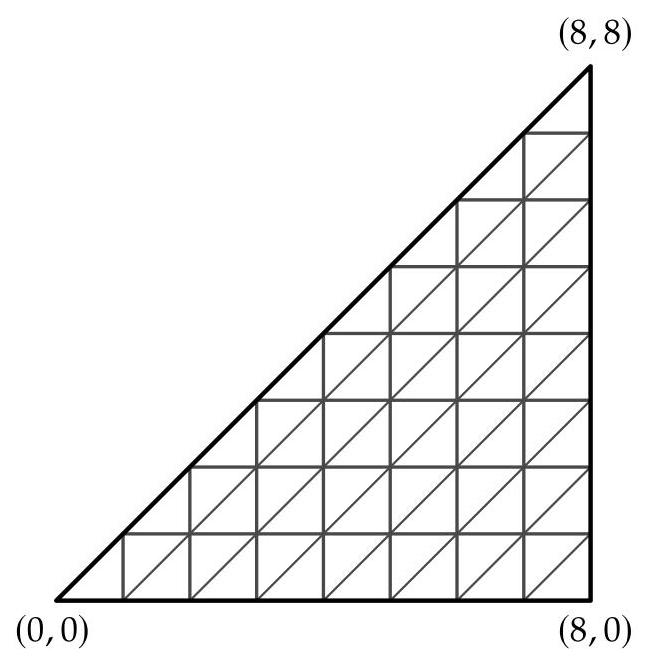
\includegraphics[width=0.5\textwidth]{images/ch07-fig18.jpg}
\caption{二维单纯形\({T}_{2}\left( k\right)\) 的弗赖登塔尔三角剖分，其顶点为 \(\left( {0,0}\right) ,\left( {k,0}\right)\) 和 \((k, k)\) ，其中 \(k = 8\) 。}
\label{fig:7.16}
\end{figure}

这些向量仿射无关，因为在 (\ref{eq:7.4}) 中考虑的 \({\mathbb{R}}^{1 + d}\) 中对应的向量 \({z}^{i} = \left( \begin{matrix} 1 \\  {v}^{i}\left( k\right)  \end{matrix}\right)\) 线性无关，因为 \(\mathop{\sum }\limits_{{i = 0}}^{d}{z}^{i}{\lambda }_{i} = \mathbf{0}\) 意味着 \({\lambda }_{d} = 0\) ，然后 \({\lambda }_{d - 1} = 0\) ，依此类推，直到 \({\lambda }_{0} = 0\) 。因此，它们的凸包定义了一个单纯形，我们称之为 \({T}_{d}\left( k\right)\) 。

设 \(k = 1\) 。 \({T}_{d}\left( 1\right)\) 的顶点是从全零向量 \({v}^{0}\) 开始定义的，每次将一个坐标从 0 变为 1，直到得到全 1 向量 \({v}^{d} = \mathbf{1} \in  {\mathbb{R}}^{d}\) 。为了构造 \({T}_{d}\left( 1\right)\) ，我们按自然顺序 \(1,\ldots ,d\) 选择坐标。作为推广，考虑坐标的任意顺序 \(\pi \left( 1\right) ,\ldots ,\pi \left( d\right)\) ，即 \(1,\ldots ,d\) 的一个排列 \(\pi\) (集合 \(\{ 1,\ldots ,d\} )\) 上的双射)。我们用 \(\operatorname{Perm}\left( d\right)\) 表示 \(1,\ldots ,d\) 的所有排列的集合。对于 \(\pi  \in  \operatorname{Perm}\left( d\right)\) ，设 \({v}_{\pi }^{0} = \mathbf{0} \in  {\mathbb{R}}^{d}\) ，对于 \(i = 1,\ldots ,d\) 定义

\begin{equation}
{v}_{\pi }^{i} = {v}_{\pi }^{i - 1} + {e}_{\pi \left( i\right) }.\label{eq:7.26}
\end{equation}

也就是说，第 \(i\) 个向量 \({v}_{\pi }^{i}\) 是通过在前一个向量上加上单位向量 \({e}_{\pi \left( i\right) }\) 得到的，这将位置 \(\pi \left( i\right)\) 处的坐标从 0 变为 1 。例如，如果 \(\left( {\pi \left( 1\right) ,\ldots ,\pi \left( d\right) }\right)  = \left( {2,3,1,4}\right)\) ，那么

\begin{equation}
{v}_{\pi }^{0} = \left( \begin{array}{l} 0 \\  0 \\  0 \\  0 \end{array}\right) ,{v}_{\pi }^{1} = \left( \begin{array}{l} 0 \\  1 \\  0 \\  0 \end{array}\right) ,{v}_{\pi }^{2} = \left( \begin{array}{l} 0 \\  1 \\  1 \\  0 \end{array}\right) ,{v}_{\pi }^{3} = \left( \begin{array}{l} 1 \\  1 \\  1 \\  0 \end{array}\right) ,{v}_{\pi }^{4} = \left( \begin{array}{l} 1 \\  1 \\  1 \\  1 \end{array}\right) .\label{eq:7.27}
\end{equation}

这定义了 \({C}_{d}\) 的顶点的一条“单调路径”，它从全零向量 0 开始，到全 1 向量 1 结束。(很容易看出，单位立方体 \({C}_{d}\) 的顶点是 \({\mathbb{R}}^{d}\) 中的 \({2}^{d}\) 个向量，其中每个分量要么是 0 要么是 1 。)这些向量的凸包定义了单纯形

\[
{T}_{d}^{\pi } = \operatorname{conv}\left\{  {{v}_{\pi }^{0},{v}_{\pi }^{1},\ldots ,{v}_{\pi }^{d}}\right\}  .
\]

以下引理用 \(d + 1\) 个线性不等式而不是顶点的凸包来描述这个单纯形。

\bigskip
\noindent
\begin{lemma}\label{lem:7.21}
设 \(x \in  {\mathbb{R}}^{d}\) 和 \(\pi  \in  \operatorname{Perm}\left( d\right)\) 。那么$x \in T^{\pi}_d$当且仅当

\begin{equation}
1 \geq  {x}_{\pi \left( 1\right) } \geq  {x}_{\pi \left( 2\right) } \geq  \cdots  \geq  {x}_{\pi \left( d\right) } \geq  0.\label{eq:7.28}
\end{equation}
\end{lemma}

\bigskip
\noindent
\begin{proof}
假设 (\ref{eq:7.28}) 成立。通过以下方式定义 \({y}_{0},{y}_{1},\ldots ,{y}_{d}\)

\[
{y}_{0} = 1 - {x}_{\pi \left( 1\right) }
\]

\[
{y}_{1} = {x}_{\pi \left( 1\right) } - {x}_{\pi \left( 2\right) }
\]

\begin{equation}
\vdots\label{eq:7.29}
\end{equation}

\[
{y}_{d - 1} = {x}_{\pi \left( {d - 1}\right) } - {x}_{\pi \left( d\right) }
\]

\[
{y}_{d} = {x}_{\pi \left( d\right) }
\]

这意味着

\[
{x}_{\pi \left( j\right) } = \mathop{\sum }\limits_{{i = j}}^{d}{y}_{i}\;\left( {1 \leq  j \leq  d}\right)
\]

并且由 (\ref{eq:7.29}) 和 (\ref{eq:7.28})

\begin{equation}
\mathop{\sum }\limits_{{i = 0}}^{d}{y}_{i} = 1,\;{y}_{i} \geq  0\;\left( {1 \leq  i \leq  d}\right) .\label{eq:7.30}
\end{equation}

由(\ref{eq:7.26})式，正如示例(\ref{eq:7.27})所示，向量 \({v}_{\pi }^{i}\) 的分量由下式给出

\[
{\left( {v}_{\pi }^{i}\right) }_{\pi \left( j\right) } = \left\{  {\begin{array}{ll} 0 & \text{ if }i < j \\  1 & \text{ if }i \geq  j \end{array}\;\left( {0 \leq  i \leq  d,1 \leq  j \leq  d}\right) .}\right.
\]

因此，由(\ref{eq:7.29})式

\[
\mathop{\sum }\limits_{{i = 0}}^{d}{\left( {v}_{\pi }^{i}\right) }_{\pi \left( j\right) }{y}_{i} = \mathop{\sum }\limits_{{i = j}}^{d}{y}_{i} = {x}_{\pi \left( j\right) }\;\left( {1 \leq  j \leq  d}\right)
\]

所以

\begin{equation}
x = \mathop{\sum }\limits_{{i = 0}}^{d}{v}_{\pi }^{i}{y}_{i}\label{eq:7.31}
\end{equation}

也就是说，由(\ref{eq:7.30})式可知， \(x\) 是向量 \({v}_{\pi }^{0},\ldots ,{v}_{\pi }^{d}\) 的凸组合，这表明 \(x \in  {T}_{d}^{\pi }\) 。此外，(\ref{eq:7.29})式中的 \({y}_{0},\ldots ,{y}_{d}\) 是 \(x\) 的重心坐标。

反之，对于 \(0 \leq  i \leq  d\) ， \({T}_{d}^{\pi }\) 的任何顶点 \(x = {v}_{\pi }^{i}\) 都满足(\ref{eq:7.28})式，其中唯一严格成立的不等式(如果 \(0 < i < d\) )是当 \(x\) 的分量从 1 变为 0 时。因此，不等式\eqref{eq:7.28}对于这些顶点的任何凸组合也成立，即对于 \({T}_{d}^{\pi }\) 的任何元素都成立。
\end{proof}
\bigskip

对于恒等排列 \(\pi\) ，单纯形 \({T}_{d}\left( 1\right)\) 是 \({T}_{d}^{\pi }\) 。容易看出 \({T}_{d}\left( k\right)  = \left\{  {{xk} \mid  x \in  {T}_{d}\left( 1\right) }\right\}\) ，因此根据引理\ref{lem:7.21}

\begin{equation}
z \in  {T}_{d}\left( k\right) \; \Leftrightarrow  \;k \geq  {z}_{1} \geq  {z}_{2} \geq  \cdots  \geq  {z}_{d} \geq  0.\label{eq:7.32}
\end{equation}

\bigskip
\noindent
\begin{lemma}\label{lem:7.22}
集合 \(\left\{  {{T}_{d}^{\pi } \mid  \pi  \in  \operatorname{Perm}\left( d\right) }\right\}\) 是单位立方体 \({C}_{d}\) 的一个三角剖分。
\end{lemma}

\bigskip
\noindent
\begin{proof}
设 \(x = {\left( {x}_{1},\ldots ,{x}_{d}\right) }^{\top } \in  {C}_{d}\) ，即对于 \(1 \leq  i \leq  d\) 有 \(1 \geq  {x}_{i} \geq  0\) ，并设 \(\pi  \in  \operatorname{Perm}\left( d\right)\) 。对 \(x\) 的分量 \({x}_{i}\) 进行排序，使得(\ref{eq:7.28})式成立(如果 \(x\) 的某些分量彼此相等，则排列 \(\pi\) 不唯一)。根据引理\ref{lem:7.21}， \(x \in  {T}_{d}^{\pi }\) 。这表明 \({C}_{d} = \mathop{\bigcup }\limits_{{\pi  \in  \operatorname{Perm}\left( d\right) }}{T}_{d}^{\pi }\) 。

如果 \(\pi ,{\pi }^{\prime } \in  \operatorname{Perm}\left( d\right)\) 且 \(\pi  \neq  {\pi }^{\prime }\) ，那么通过选取(\ref{eq:7.28})式中某些严格不等式对应的 \(x \in  {T}_{d}^{\pi }\) (显然 \(x \notin  {T}_{d}^{{\pi }^{\prime }}\) )，有 \({T}_{d}^{\pi } \nsubseteq  {T}_{d}^{{\pi }^{\prime }}\) 。还需证明任意两个子单纯形 \({T}_{d}^{\pi }\) 和 \({T}_{d}^{{\pi }^{\prime }}\) 的交集是它们两者的一个面。 \({T}_{d}^{\pi } \cap  {T}_{d}^{{\pi }^{\prime }}\) 中的任何 \(x\) 都满足(\ref{eq:7.28})式以及

\begin{equation}
{x}_{{\pi }^{\prime }\left( 1\right) } \geq  {x}_{{\pi }^{\prime }\left( 2\right) } \geq  \cdots  \geq  {x}_{{\pi }^{\prime }\left( d\right) }.\label{eq:7.33}
\end{equation}

任何在(\ref{eq:7.28})和(\ref{eq:7.33})中反向成立的不等式都必须以等式形式成立。这包括任何隐含的等式；例如，如果对于 \(d = 3\) 我们有 \({x}_{1} \geq  {x}_{2} \geq  {x}_{3}\) 和 \({x}_{2} \geq  {x}_{3} \geq  {x}_{1}\) ，那么这意味着 \({x}_{1} = {x}_{3}\) 以及 \({x}_{2} = {x}_{3}\) 。交集 \({T}_{d}^{\pi } \cap  {T}_{d}^{{\pi }^{\prime }}\) 随后由(\ref{eq:7.28})表征，其中一些不等式被等式取代。在(\ref{eq:7.29})中 \(x\) 的与这些等式对应的重心坐标 \({y}_{1},\ldots ,{y}_{d - 1}\) 随后被设为零，这意味着在(\ref{eq:7.31})中 \(x\) 的表示不使用相应的顶点。因此， \(x\) 只是剩余顶点的凸组合。这些是 \({T}_{d}^{\pi } \cap  {T}_{d}^{{\pi }^{\prime }}\) 的顶点，因此它是两个子单纯形 \({T}_{d}^{\pi }\) 和 \({T}_{d}^{{\pi }^{\prime }}\) 的公共面，正如所声称的那样。可能会出现(\ref{eq:7.28})中的所有不等式都是等式的情况，使得公共面只有顶点0和1。
\end{proof}
\bigskip

数字 \(1,\ldots ,d\) 有 \(d\) ! 种排列\(\pi\) 。任意两个单纯形 \({T}_{d}^{\pi }\) 和 \({T}_{d}^{{\pi }^{\prime }}\) 具有相同的形状和大小，因为它们仅在坐标顺序上有所不同，并且它们的交集是一个维度为 \(d - 1\) 或更低的集合，该集合在 \({\mathbb{R}}^{d}\) 中的体积为零。由于单位立方体\({C}_{d}\) 的体积为1，引理\ref{lem:7.22}意味着每个单纯形 \({T}_{d}^{\pi }\) 的体积为 \(\frac{1}{d!}\) 。

现在，我们使用引理\ref{lem:7.22}中单位立方体 \({C}_{d}\) 的三角剖分来构造(\ref{eq:7.25})中单纯形 \({T}_{d}\left( k\right)\) 的三角剖分，其中 \(k \geq  1\) 为某个整数。

对于 \({\mathbb{R}}^{d}\) 中的有界多面体 \(P\) ，例如 \({C}_{d}\) 或 \({T}_{d}^{\pi }\) ，以及一个整数“网格”向量 \(g =\)  \({\left( {g}_{1},\ldots ,{g}_{d}\right) }^{\top } \in  {\mathbb{Z}}^{d}\) ，设 \(g + P = \{ g + x \mid  x \in  P\}\) 。设

\begin{equation}
\sum  = \left\{  {g + {T}_{d}^{\pi } \mid  \pi  \in  \operatorname{Perm}\left( d\right) ,g \in  {\mathbb{Z}}^{d},g + {T}_{d}^{\pi } \subseteq  {T}_{d}\left( k\right) }\right\}  .\label{eq:7.34}
\end{equation}

换句话说，我们考虑 \({C}_{d}\) 的三角剖分中的任意单纯形 \({T}_{d}^{\pi }\) ，通过加上某个整数向量 \(g\) 对其进行平移，如果得到的集合 \(g + {T}_{d}^{\pi }\) 是 \({T}_{d}\left( k\right)\) 的子集，那么这就是 \(\sum\) 中的一个子单纯形。根据(\ref{eq:7.32})，只有当 \(0 \leq  {g}_{i} \leq  k\) 对于 \(1 \leq  i \leq  d\) 成立时才会这样，因为否则 \(g + \mathbf{0} \notin  {T}_{d}\left( k\right)\) (其中 \(\mathbf{0} \in  {T}_{d}^{\pi }\) )，所以 \(\sum\) 是有限的。图\ref{fig:7.17}展示了 \(\sum\) 在 \(d = 3\) 和 \(k = 2\) 时的情况。

\begin{figure}[htbp]
\centering
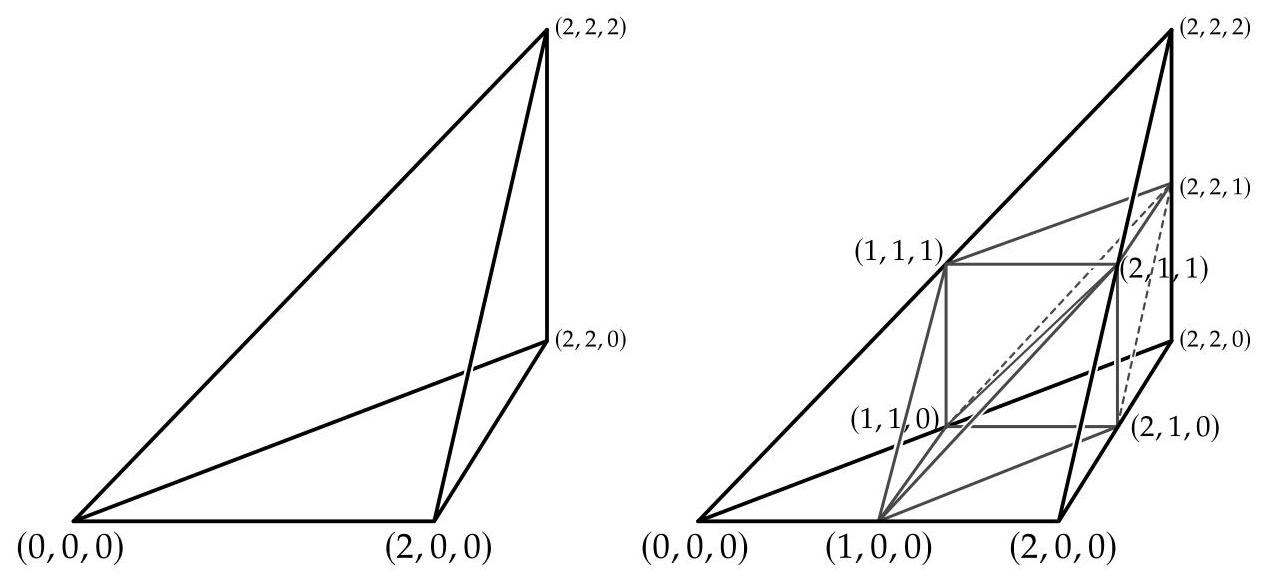
\includegraphics[width=0.9\textwidth]{images/ch07-fig19.jpg}
\caption{三维单纯形 \({T}_{3}\left( k\right)\) 的弗赖登塔尔三角剖分 \(\sum\) ，其顶点为 \(\left( {0,0,0}\right) ,\left( {k,0,0}\right) ,\left( {k,k,0}\right)\) 以及对于 \(k = 2\) 的 $(k, k, k)$。}
\label{fig:7.17}
\end{figure}

\bigskip
\noindent
\begin{theorem}\label{theo:7.23}
如 (\ref{eq:7.34}) 所定义的 \(\sum\) 是 \({T}_{d}\left( k\right)\) 的一个三角剖分。
\end{theorem}

\bigskip
\noindent
\begin{proof}
由 (\ref{eq:7.34}) 可知， \(\mathop{\bigcup }\limits_{{S \in  \sum }}S \subseteq  {T}_{d}\left( k\right)\) 。为证明反向包含关系，设 \(z \in  {T}_{d}\left( k\right)\) 。我们要找到 \(g \in  {\mathbb{Z}}^{d}\) 和 \(\pi  \in  \operatorname{Perm}\left( d\right)\) 使得 \(z \in  g + {T}_{d}^{\pi }\) ，并且至关重要的是，满足 (\ref{eq:7.34}) 中要求的 \(g + {T}_{d}^{\pi } \subseteq  {T}_{d}\left( k\right)\) 。如果这成立，那么对于某个 \(x \in  {T}_{d}^{\pi }\) 有 \(z = g + x\) ，这意味着

\begin{equation}
{z}_{i} = {g}_{i} + {x}_{i}\;\left( {{g}_{i} \in  \mathbb{Z},{x}_{i} \in  \left\lbrack  {0,1}\right\rbrack  ,1 \leq  i \leq  d}\right) .\label{eq:7.35}
\end{equation}

在 (\ref{eq:7.35}) 中，如果 \({z}_{i} \in  \mathbb{Z}\) ， \({g}_{i}\) 和 \({x}_{i}\) 的选择不是唯一的，因为此时 \({x}_{i} = 0\) 或 \({x}_{i} = 1\) 都是可能的。那么我们通常选择 \({x}_{i} = 0\) ，除非当 \({z}_{i} = k\) 时我们选择 \({g}_{i} = k - 1\) 和 \({x}_{i} = 1\) ，以确保 \(g + {T}_{d}^{\pi } \subseteq  {T}_{d}\left( k\right)\) 。对于 \(\left\lfloor  {z}_{i}\right\rfloor   = \max \left\{  {t \in  \mathbb{Z} \mid  t \leq  {z}_{i}}\right\}\) ，这可通过

\begin{equation}
{g}_{i} = \left\{  {\begin{array}{ll} \left\lfloor  {z}_{i}\right\rfloor  & \text{ if }{z}_{i} < k \\  k - 1 & \text{ if }{z}_{i} = k, \end{array}\;{x}_{i} = {z}_{i} - {g}_{i}\;\left( {1 \leq  i \leq  d}\right) ,}\right.\label{eq:7.36}
\end{equation}

这显然意味着 (\ref{eq:7.35})。

类似地， \({z}_{i}\) 的整数部分 \({g}_{i}\) 满足

\begin{equation}
{g}_{i} \geq  {g}_{i + 1}\;\left( {1 \leq  i < d}\right)\label{eq:7.37}
\end{equation}

因为如果 \({z}_{i} = k\) ，那么 \({z}_{i + 1} \leq  k\) 且 \({g}_{i} = k - 1 \geq  {g}_{i + 1}\) ，并且如果 \({z}_{i} < k\) ，那么由 (\ref{eq:7.36}) 我们有 \({x}_{i} < 1\) ，使得 \({g}_{i} < {g}_{i + 1}\) 意味着 \({z}_{i} = {g}_{i} + {x}_{i} < {g}_{i} + 1 \leq  {g}_{i + 1} \leq  {z}_{i + 1}\) ，这与 (\ref{eq:7.32}) 矛盾。

给定式\eqref{eq:7.35}，我们希望找到 \(\pi  \in  \operatorname{Perm}\left( d\right)\) 使得 \(x \in  {T}_{d}^{\pi }\) 且 \(g + {T}_{d}^{\pi } \subseteq  {T}_{d}\left( k\right)\) 。第二个条件并非自动满足:例如，如果 \(d = 2\) 且 \(k = 1\) ，那么 \(\sum  = \left\{  {{T}_{2}\left( 1\right) }\right\}\) ，并且对于 \(z = x = \left( {\frac{1}{2},\frac{1}{2}}\right)\) ， \({T}_{2}\left( 1\right)\) 和 \({T}_{2}^{\pi }\left( 1\right)\) 在 \(\left( {\pi \left( 1\right) ,\pi \left( 2\right) }\right)  = \left( {2,1}\right)\) 时都包含 \(x\) ，但 \(\mathbf{0} + {T}_{2}^{\pi }\left( 1\right)  \notin  \sum\) 。以下是 \(\pi\) 的一个稳妥选择。用一个排列 \(\pi\) 对 \(x\) 的分量 \({x}_{i}\) 进行排序，使得式\eqref{eq:7.28}成立，并且使得

\begin{equation}
1 \leq  h < j \leq  d,\;{x}_{\pi \left( h\right) } = {x}_{\pi \left( j\right) }\; \Rightarrow  \;\pi \left( h\right)  < \pi \left( j\right) .\label{eq:7.38}
\end{equation}

这总能实现，如有必要，若 \({x}_{\pi \left( h\right) } =\)  \({x}_{\pi \left( j\right) }\) ，可交换 \(\pi \left( h\right)\) 和 \(\pi \left( j\right)\) ，这能保持式\eqref{eq:7.28}成立。然后根据引理\ref{lem:7.21} 有 \(x \in  {T}_{d}^{\pi }\) 。我们想证明对于任意 \(y \in  {T}_{d}^{\pi }\) 都有 \(g + y \in  {T}_{d}\left( k\right)\) ，即根据式\eqref{eq:7.32}

\begin{equation}
{g}_{i} + {y}_{i} \geq  {g}_{i + 1} + {y}_{i + 1}\;\left( {1 \leq  i < d}\right)\label{eq:7.39}
\end{equation}

(由(\ref{eq:7.36})，我们有 \(k \geq  {g}_{1} + {y}_{1}\) 和 \({g}_{d} + {y}_{d} \geq  0\) )。由(\ref{eq:7.37})，若 \({y}_{i} \geq  {y}_{i + 1}\) ，则条件(\ref{eq:7.39})成立。否则，令 \(y \in  {T}_{d}^{\pi }\) ，并假设对于某个 \(1 \leq  i < d\) 有 \({y}_{i} < {y}_{i + 1}\) 。令 \(i + 1 = \pi \left( h\right)\) 且 \(i = \pi \left( j\right)\) 。那么 \({y}_{\pi \left( h\right) } = {y}_{i + 1} > {y}_{i} = {y}_{\pi \left( j\right) }\) ，根据引理\ref{lem:7.21}这意味着 \(h < j\) 。接着 \({x}_{\pi \left( h\right) } \geq  {x}_{\pi \left( j\right) }\) ，其中 \({x}_{\pi \left( h\right) } = {x}_{\pi \left( j\right) }\) 由(\ref{eq:7.38})将意味着 \(i + 1 = \pi \left( h\right)  <\)  \(\pi \left( j\right)  = i\) ，而这是不可能的，即 \({x}_{i + 1} = {x}_{\pi \left( h\right) } > {x}_{\pi \left( j\right) } = {x}_{i}\) 。由(\ref{eq:7.37})，要么 \({g}_{i} = {g}_{i + 1}\) ，要么 \({g}_{i} > {g}_{i + 1}\) 。若 \({g}_{i} = {g}_{i + 1}\) ，则 \({z}_{i + 1} = {g}_{i + 1} + {x}_{i + 1} > {g}_{i} + {x}_{i} = {z}_{i}\) ，这与(\ref{eq:7.32})矛盾。因此， \({g}_{i} + {y}_{i} \geq  {g}_{i} \geq  {g}_{i + 1} + 1 \geq  {g}_{i + 1} + {y}_{i + 1}\) 。这表明了(\ref{eq:7.39})，因此，如所声称的， \(g + {T}_{d}^{\pi } \subseteq  {T}_{d}\left( k\right)\) 。也就是说， \(\sum\) 中的子单形覆盖 \({T}_{d}\left( k\right)\) 。

为了证明 \(\sum\) 是 \({T}_{d}\left( k\right)\) 的一个三角剖分，还需证明没有子单纯形是另一个子单纯形的子集，并且两个子单纯形的交集是两者的一个面。这两个性质的证明与引理\ref{lem:7.22}类似，若 \(g = {g}^{\prime }\) ，则该引理对两个子单纯形 \(g + {T}_{d}^{\pi }\) 和 \({g}^{\prime } + {T}_{d}^{{\pi }^{\prime }}\) 成立。若 \(g \neq  {g}^{\prime }\) ，则这两个子单纯形是两个不同立方体 \(g + {C}_{d}\) 和 \({g}^{\prime } + {C}_{d}\) 的子集，这两个立方体的非空内部不相交，因此没有一个子单纯形是另一个的子集。 \(g + {T}_{d}^{\pi }\) 和 \({g}^{\prime } + {T}_{d}^{{\pi }^{\prime }}\) 的交集是 \(\left( {g + {C}_{d}}\right)  \cap  \left( {{g}^{\prime } + {C}_{d}}\right)\) 的子集，仅当对于 \(1 \leq  i \leq  d\) 有 \(\left| {{g}_{i} - {g}_{i}^{\prime }}\right|  \leq  1\) 时，该交集才非空。根据引理\ref{lem:7.21}，当且仅当 \(z = g + x = {g}^{\prime } + {x}^{\prime }\) 时 \(z \in  \left( {g + {T}_{d}^{\pi }}\right)  \cap  \left( {{g}^{\prime } + {T}_{d}^{{\pi }^{\prime }}}\right)\) ，从而 (\ref{eq:7.28}) 成立，并且类似地

\begin{equation}
1 \geq  {x}_{{\pi }^{\prime }\left( 1\right) }^{\prime } \geq  {x}_{{\pi }^{\prime }\left( 2\right) }^{\prime } \geq  \cdots  \geq  {x}_{{\pi }^{\prime }\left( d\right) }^{\prime } \geq  0.\label{eq:7.40}
\end{equation}

若 \({g}_{i} = {g}_{i}^{\prime } + 1\) ，则方程 \({z}_{i} = {g}_{i} + {x}_{i} = {g}_{i}^{\prime } + {x}_{i}^{\prime }\) 施加了额外的方程 \({x}_{i} = 1\) 和 \({x}_{i}^{\prime } = 0\) (类似地，若 \({g}_{i} + 1 = {g}_{i}^{\prime }\) ，则有 \({x}_{i} = 0\) 和 \({x}_{i}^{\prime } = 1\) )。对于那些满足 \({g}_{i} = {g}_{i}^{\prime }\) 的下标 \(i\) ，我们有 \({x}_{i} = {x}_{i}^{\prime }\) ，如果 \(x\) 和 \({x}^{\prime }\) 的这些分量在这些不等式中以相反顺序出现，那么这会在 (\ref{eq:7.28}) 和 (\ref{eq:7.40}) 中引出更多方程。正如在引理\ref{lem:7.22}的证明中所论述的，这些方程意味着 (\ref{eq:7.29}) 中某些重心坐标 \({y}_{0},{y}_{1},\ldots ,{y}_{d}\) 为零(如果 \({x}_{\pi \left( 1\right) } = 1\) ，现在可能包括 \({y}_{0}\) ；如果 \({x}_{\pi \left( d\right) } = 0\) ，可能包括 \({y}_{d}\) )，这就将两个子单纯形的相应顶点排除在它们的交集之外。剩下的顶点(如果有的话)就是交集的顶点，因此该交集是两个子单纯形的公共面。这就完成了三角剖分性质的证明。
\end{proof}
\bigskip

单纯形 \({T}_{d}\left( k\right)\) 在 (\ref{eq:7.25}) 中有 \(d + 1\) 个顶点 \({v}^{i}\left( k\right)\) ，这些顶点是 \({\mathbb{R}}^{k}\) 中边长为 \(k\) 的立方体的顶点。(\ref{eq:7.34}) 中的三角剖分 \(\sum\) 将 \({T}_{d}\left( k\right)\) 细分为单纯形 \({T}_{d}^{\pi }\) (这些单纯形对单位立方体 \({C}_{d}\) 进行三角剖分)，并通过整数向量 \(g \in  {\mathbb{Z}}^{d}\) 进行平移。目标是得到单位单纯形 \(\Delta\) 的任意精细的三角剖分，如 KKM 引理(定理\ref{theo:7.12})中所使用的那样。这可以通过以下方式实现:当使用引理\ref{lem:7.3} 中的仿射双射 \(J\) 将 \({T}_{d}\left( k\right)\) 映射到 \(\Delta\) 时，我们得到 \(\Delta\) 的相应三角剖分 \(\{ J\left( T\right)  \mid  T \in  \sum \}\) 。对于该三角剖分的每个子单纯形 \(J\left( {g + {T}_{d}^{\pi }}\right)\) ，其顶点之间距离的最大值仅取决于 \(\pi\) ，而不取决于 \(g\) 。该最大值(在所有 \(\pi  \in  \operatorname{Perm}\left( d\right)\) 和所有顶点对上)与 \(\frac{1}{k}\) 成正比，因为 \(J\) 是仿射的且 \({T}_{d}\left( k\right)  = \left\{  {{xk} \mid  x \in  {T}_{d}\left( 1\right) }\right\}\) 。因此，对于任何 \(\varepsilon  > 0\) ，可以选择足够大的 \(k\) ，使得 \(\Delta\) 的三角剖分的任何子单纯形中的任意两点之间的距离都不大于 \(\varepsilon\) ，这就得到了所需的 \(\varepsilon\) - 精细三角剖分。 

布劳威尔不动点定理\ref{theo:7.20} 的证明至此完成。

\section{延伸阅读}\label{sec-7.8}

不动点定理在布劳威尔(1911 年，命题 4)的论文结尾处被提出。在这篇以及相关论文中，布劳威尔发展并使用了连续函数的单纯逼近的“度”(一个点的原像数量)的概念。详细讨论见布劳威尔(1976 年)。关于布劳威尔不动点定理及其后续扩展的广泛影响的历史综述见帕克(1999 年)。

布劳威尔不动点定理是拓扑学中的一个重要定理。拓扑学的基本概念是连续性，但更本质地说，拓扑学可以被视为对“位置”的定性研究。在这方面发表的第一篇论文是欧拉(1741 年)对“哥尼斯堡七桥问题”的解答(另见比格斯、劳埃德和威尔逊，1976 年)。欧拉的论文标志着图论和拓扑学的基础；它引入了图的概念，并且节点的度起着核心作用。斯佩纳引理与图中奇数度节点的偶数性相关是恰当的。

定理\ref{theo:7.10} 归功于斯佩纳(1928 年)，并且被克纳斯特、库拉托夫斯基和马祖尔克维奇(1929 年)用于借助他们的定理\ref{theo:7.12} 证明单纯形上的不动点定理。正如我们在定理\ref{theo:7.10} 的证明中所提到的，这些证明使用了方程 (\ref{eq:7.12}) 中的模 2 计数。“奇偶性论证”这一术语由帕帕迪米特里欧(1994 年)创造。

路径跟踪的论证归功于科恩(Cohen，1967)。科恩的证明没有提供足够详细的内容，让人无法看到路径也可能回到低几个维度的情况，如图\ref{fig:7.10}中的示例所示。更精确的描述请参阅库恩(Kuhn，1969)。我们将图的“内部”节点定义为 \({C}^{\prime }\) 中的子极面，而不是(\ref{eq:7.11})中 \(A\) 的元素。当处于固定维度时，更自然的做法是仅将单纯剖分中的子单纯形，即 \(D\) 和 \(A\) 的元素，视为图的节点，如果它们在 \({C}^{\prime }\) 中有一个公共子极面，则用一条边将它们连接起来。然而，特别是对于 \({G}_{2}\) 的构造，边更容易被看作线段，节点更容易被看作 \({\sum }_{2}\) 中的顶点。(\ref{eq:7.13})中 \(G\) 构造的一个关键论证是，图 \({G}_{n}\) 中某些路径的端点具有不同的维度，并且我们仅在端点处转换到更高的维度。

用于证明波尔查诺 - 魏尔施特拉斯定理的“海景酒店”的例子取自布莱恩特(Bryant，1990)。

弗罗伊登塔尔单纯剖分归功于弗罗伊登塔尔(Freudenthal，1942)，并且被多次重新发现，例如库恩(Kuhn，1960)。

\section{第7章练习}\label{sec-7.9}

\bigskip
\noindent
\begin{exercise}\label{exer:7.1}
设 \(C = \left\{  {\left( {x,y}\right)  \in  {\mathbb{R}}^{2} \mid  {x}^{2} + {y}^{2} \leq  1}\right\}\) ，并考虑以下函数 \(g,h,f : C \rightarrow  C\) :

\[
g\left( {x,y}\right)  = \left( {x,\sqrt{1 - {x}^{2}}}\right) ,\;h\left( {x,y}\right)  = \left( {-y,x}\right) ,\;f\left( {x,y}\right)  = h\left( {g\left( {x,y}\right) }\right) .
\]

设 \(G = g\left( C\right)  = \{ g\left( {x,y}\right)  \mid  \left( {x,y}\right)  \in  C\}\) 。描述 \(C\) 和 \(G\) 的几何形状，以及函数 \(g\) 和 \(h\) 的作用方式。每个函数 \(g,h,f\) 在 \(C\) 中是否有不动点？说明原因。如果有，确定 \(g,h\) 和 \(f\) 每个函数的所有不动点。
\end{exercise}

\bigskip
\noindent
\begin{exercise}\label{exer:7.2}
对于一般的有界多面体 \(P\) ， \(P\) 的顶点被定义为 \(P\) 的极点，即它不是 \(P\) 中其他点的凸组合。

(a)证明对于由仿射无关点 \({v}^{1},\ldots ,{v}^{d}\) 的凸包给出的单纯形 \(S\) ，根据这个定义，每个点 \({v}^{i}\) 确实是 \(S\) 的一个顶点。

(b)证明单纯形的顶点集是唯一的。
\end{exercise}

\bigskip
\noindent
\begin{exercise}\label{exer:7.3}
给出以下例子

(a)两个单纯形，它们的交集不是单纯形；

(b)一个非空凸集，它没有极点；

(c)一个有界凸集，它至少有一个极点，但它不等于其极点的凸包。
\end{exercise}

\bigskip
\noindent
\begin{exercise}\label{exer:7.4}
证明以下斯佩纳引理(定理\ref{theo:7.10})的推广是错误的:设 \(S\) 是一个顶点为 \({v}^{1},\ldots ,{v}^{d}\) 的单纯形，设 \(\sum\) 是 \(S\) 的一个三角剖分，并考虑 \(V\) 中顶点的一个标签，使得 \({v}_{i}\) 具有标签 \(i\) ，其中 \(1 \leq  i \leq  d\) 。那么 \(\sum\) 至少有一个完全标记的子单纯形。

\end{exercise}
